\chapter{Implementation and Concrete Algorithm Components}\label{ch:impl}

% [SKELETON] Detail focus. After a brief known SOTA, each PRT-ART algorithm as a figure + description;
% then axis implementation (one overall-concept figure per axis) and all levels of the measurement system.

This chapter descends into detail: first the repository architecture with the carrier-stage chain
(Section~\ref{sec:anatomy-levels}) and the four work modes of a permutation, then each key point of
PRT-ART individually and visually, next the axis implementation together with the \emph{one} architecture
in code, the code shape of the build chain, the levels E4--E0 in code and the contract surfaces at the
carrier binaries, after that the quality assurance via contract tests per layer including the two-gate
protocol and the code shape of the realm roots --- system and measurement axes including the hardware
detection --- and finally the register of design patterns, the hybrid stage and the store. At its core,
the \emph{one} architecture is a self-optimizing compiler-compiler structure: the planner generates the
build orders from the user XML, the builder generates the compiled artefacts from them, and the evaluation
of the measured values feeds the next planning (Section~\ref{sec:mess-chain}). The apparatus thus stands
in the line of the empirical autotuning systems that generate candidate implementations, measure them and
make the selection from the measured
values~\cite{whaley2001atlas,frigo1998fftw,ansel2014opentuner,balaprakash2018autotuning}; the difference
is that here it is not the parameters of a fixed implementation that are permuted but the organ assignment
of a living being, and a separate binary is generated per permutation.

\section{Four-Repository Architecture}\label{sec:repos}
The implementation is distributed across four Git repositories with clearly separated responsibilities:
\begin{itemize}
  \item \texttt{comdare-cache-engine} --- \textbf{how} measurement is done: the building-block library and
  the builder (XML config parser,
  \texttt{generate\_\allowbreak{}module\_\allowbreak{}from\_\allowbreak{}profile} code generation,
  permutation loop, module loader, the seven-phase \texttt{ExperimentDriver} with the phases
  \texttt{phase1\_enumerate} to \texttt{phase7\_export} and the experiment planner
  \texttt{ExperimentPlanDirector}, Section~\ref{sec:impl-pipeline}); the ABI headers under \texttt{abi/}
  --- the living ABI core \texttt{module\_\allowbreak{}abi\_\allowbreak{}v1} as well as the test cluster,
  isolated from the build, of \texttt{baustein\_\allowbreak{}variants} and
  \texttt{resolve\_\allowbreak{}baustein} (Section~\ref{sec:axes-impl}) ---; the 33~SOTA profiles under
  \texttt{algorithm\_\allowbreak{}profiles/\allowbreak{}sota} as executable XML --- 30~full profiles and
  three abstract profiles (Section~\ref{sec:sota-instances}) --- and the test suites. The library
  \texttt{search\_\allowbreak{}engine} is a declared, content-empty skeleton (seventeen files, eight of
  them placeholders and nine build descriptions without source code), and
  \texttt{execution\_\allowbreak{}engine} contains three content files (result aggregator and experiment
  demonstration); the living root of the execution engine lies under
  \texttt{libs/\allowbreak{}cache\_\allowbreak{}engine/\allowbreak{}execution\_\allowbreak{}engine}
  (Section~\ref{sec:impl-architecture}). The source tree follows a Pitchfork layout (\texttt{apps/} for
  executables, \texttt{libs/} for libraries, \texttt{libs/common} for cross-cutting code); added to these
  are \texttt{libs/traeger} with the four carrier stages (below),
  \texttt{libs/\allowbreak{}cache\_\allowbreak{}engine/\allowbreak{}heuristik} with six headers (axis
  spline, break-even, measurement-curve loader, offline clustering of the workloads, feature vector,
  optimization catalogue) and \texttt{libs/test\_infra} (benchmark suite, workload generator, test data).
  \item \texttt{comdare-prt-art} --- the \textbf{probe}: the hybrid \texttt{PrtArtSearchEngine} with the
  1/2/N parameter rule (one parameter demands the function interfaces of a vector, two those of a map,
  more than two those of a map onto a tuple), its ABI adapters and its building blocks (4+1+2 allocator
  pools --- seven pools: four page pools with the roles trie hull, dense pages, MultiLevel and decision
  span, one rest pool and two value pools for static and dynamic values ---, OLC with reserved blocks,
  MultiLevel layout, path-oriented prefetch, DensityTracker, hypothesis metrics H1/H2/H3) as well as the
  probe-side comparison re-implementations of the rank-2/3 works (\texttt{legacy\_\allowbreak{}reimpl},
  fourteen directories P11--P27 without P15, P20 and P25), which are compared against the actual adapters
  of the cache engine in the SOTA admission test --- rank~1 (centrality rank, Section~\ref{sec:rqs})
  comprises the eight independent search designs --- all with public source code and original adapter ---
  as well as the works P08 and P09 that enter as organs; of the rank-2/3 works, P20, P25, P29 and P30
  likewise possess original adapters via \texttt{ext/}, the fourteen works in
  \texttt{legacy\_\allowbreak{}reimpl} are re-implemented from the publication without public source code
  (Section~\ref{sec:sota-instances}). Pool, prefetch and layout components are descriptor skeletons
  without a memory backend of their own; which probe building blocks reach the measurement apparatus is
  decided by the slot assignment (Section~\ref{sec:prtart-impl}).
  \item \texttt{probst-Diplomarbeit-cache-engine} --- \textbf{what} is tested by the user: the experiment
  configurations (XML together with the XSD schema), the measurement driver \texttt{messung\_driver}
  (binary \texttt{comdare-messung-driver}, the CEB role) and the evaluation toolchain of nine numbered
  programs from \texttt{01\_\allowbreak{}sample\_\allowbreak{}data\_\allowbreak{}generator} to
  \texttt{09\_\allowbreak{}tex\_\allowbreak{}formatter}
  (Figure~\ref{fig:toolchain}).
  \item the \textbf{manuscript repository} --- the versioned experiment execution directly in the
  document: the generator output of the toolchain (table and diagram files per measurement series) is
  committed under \texttt{anhang/<language>/tabellen/} and included by the manuscript, the repository has
  its own CI with the jobs \texttt{lint:secrets}, \texttt{lint:latex} and \texttt{thesis:pdf}, and the
  project repository triggers the manuscript build after a measurement run (\texttt{trigger:thesis}). A
  measured value in the document is thus a versioned artefact state with provenance, not a copied number
  --- that is the reason why the manuscript is a Git repository of its own with its own pipeline.
\end{itemize}
The fourfold order of the code is not the repository boundary but the \emph{carrier-stage chain}
planner $\to$ CEB $\to$ tier $\to$ hybrid (Section~\ref{sec:anatomy-levels}): the stamp contract knows
exactly four carriers in this order, and the source tree maps them under \texttt{libs/traeger} as four
subprojects in stage form --- \texttt{comdare\_planner}, \texttt{comdare\_ceb},
\texttt{comdare\_tier\_emission} and \texttt{comdare\_hybrid} ---, where stage $N+1$ depends only on
stage $N$, never the reverse, and each stage closes onto its predecessor stage with a strict
configuration check. Implementation status of this order: the subprojects form a scaffold (per stage a
build description and a description file, planner and CEB with an include directory of their own), and
the actual implementation lies as a monolith under \texttt{libs/\allowbreak{}cache\_\allowbreak{}engine};
its partition along the stages is planned but not implemented. The probe is not a stage but the
transversal supplier of organ building blocks; builder and CacheEngine share the engine repository ---
the builder as an executable (\texttt{apps/}) on top of its builder library
(\texttt{libs/\allowbreak{}cache\_\allowbreak{}engine/\allowbreak{}builder}), the CacheEngine as a library
(\texttt{libs/\allowbreak{}cache\_\allowbreak{}engine}). The stage chain is at the same time the layer at
whose binaries the contracts are partitioned into surfaces (Section~\ref{sec:impl-pipeline});
Figure~\ref{fig:traeger-stufen} shows it with its binaries, legend forms and surfaces.
\begin{figure}[htbp]\centering
\begin{tikzpicture}[font=\footnotesize,>=Stealth,
  st/.style={draw,rounded corners,fill=blue!7,minimum width=3.75cm,minimum height=3.9cm,text width=3.55cm,align=center,inner sep=3pt},
  fl/.style={draw,rounded corners,fill=orange!10,minimum width=3.75cm,minimum height=1.35cm,text width=3.55cm,align=center,inner sep=2pt,font=\tiny}]
  \node[st] (s1) at (0,0){\textbf{Stage 1: planner}\\{\tiny\texttt{comdare-experiment-planner}}\\[2pt]{\tiny resolves the user XML against the three catalogues; director walk; legend \texttt{ceb:build:\allowbreak[a,b,c]}}};
  \node[st] (s2) at (3.95,0){\textbf{Stage 2: CEB}\\{\tiny\texttt{comdare-messung-driver}}\\[2pt]{\tiny carries the measurement choice compiled in, permutes system $\times$ organ; legend per host \texttt{tier:build-batch:\allowbreak<host>}, attestations \texttt{zelle=\allowbreak[d,e,f]\allowbreak[g,h,i]}}};
  \node[st] (s3) at (7.9,0){\textbf{Stage 3: tier}\\{\tiny\texttt{comdare\_perm\_<fp>.so}}\\[2pt]{\tiny one organ permutation per binary; seven mandatory symbols; measurement batch per host \texttt{measure:\allowbreak[a,b,c]:\allowbreak batch:\allowbreak<host>}, measurement attestations \texttt{zelle=\allowbreak[a,b,c]\allowbreak[d,e,f]\allowbreak[g,h,i]}}};
  \node[st] (s4) at (11.85,0){\textbf{Stage 4: hybrid}\\{\tiny hybrid \texttt{.so}}\\[2pt]{\tiny the same mandatory symbols; dock array with docked tiers; \texttt{genus()} reports the target genus}};
  \draw[->,thick] (s1)--(s2); \draw[->,thick] (s2)--(s3); \draw[->,thick] (s3)--(s4);
  \node[fl] (f1) at (0,-2.95){Surface 2 (stamp): self-version X.Y.Z, fingerprint SHA-256, overall stamp};
  \node[fl] (f2) at (3.95,-2.95){Surface 2 (stamp): measurement and system line, fingerprint SHA-512; own measurement-gate assignment};
  \node[fl] (f3) at (7.9,-2.95){Surfaces 1--3: genus interface, stamp (three lines), measurement cut-through \texttt{IMessVisitor}};
  \node[fl] (f4) at (11.85,-2.95){Surfaces 1--3 as for the tier, plus the attached stamp lines (runtime hook)};
  \draw[dashed,gray] (s1)--(f1); \draw[dashed,gray] (s2)--(f2); \draw[dashed,gray] (s3)--(f3); \draw[dashed,gray] (s4)--(f4);
\end{tikzpicture}
\caption[The carrier-stage chain in code]{The carrier-stage chain in code: four carriers in fixed order (stamp contract), per stage the
binary, its legend form in the emitted pipeline and the contract surfaces expressed at it.
Stage $N+1$ depends only on stage $N$; only the measurement attestations contain all three axis brackets.
The surfaces partition the contracts (Section~\ref{sec:impl-pipeline}); the subprojects under
\texttt{libs/traeger} are a scaffold, the implementation lies as a monolith under
\texttt{libs/cache\_engine}.}\label{fig:traeger-stufen}
\end{figure}
Across this, the terminology separates two engine terms that must not be short-circuited. The
\texttt{CacheEngine} (\texttt{libs/\allowbreak{}cache\_\allowbreak{}engine}) is the \emph{library of axis
building blocks}: per axis it provides the interchangeable design constituents as concept/CRTP
components\footnote{CRTP\@: the \emph{Curiously Recurring Template Pattern}~\cite{coplien1995crtp}, the
static polymorphism in which a class derives from a class template to which it passes itself as the
template argument (Section~\ref{sec:software-means}); virtual calls are thereby replaced by statically
resolved ones.} and contains \emph{no} measurement logic. The \texttt{ExecutionEngine}, by contrast, is
the \emph{execution and measurement infrastructure} lying across all axes: its abstract measurable root
is \texttt{IExecutionEngine} (Section~\ref{sec:measurement-system}) with the three engine kinds Anatomy,
Virus and Hybrid; the concrete runtime adapter \texttt{SearchAlgorithmAbiAdapter<A>} provides, via the
\texttt{SearchAlgorithmAnatomy}, the OS primitives (cache-line-aligned allocation, NUMA-conformant
read pinning, coherence-aware writing); the measurement and observer couplings of the adapter are
switched via \texttt{COMDARE\_\allowbreak{}MEASUREMENT\_\allowbreak{}ON}, and the measurement aggregator
is kept host-side by the \texttt{ExperimentDriver}; the CMake option
\texttt{COMDARE\_\allowbreak{}EXPERIMENT\_\allowbreak{}MODE} marks experiment compiles and encodes at
compile time the invariant that an experiment build is always a measurement build --- it does not
itself switch any hooks, and an experiment build without measurement mode breaks the configuration. In
short: the \texttt{CacheEngine} supplies the \emph{building blocks}, the \texttt{ExecutionEngine} the
\emph{tools}; this separation keeps the production path measurement-free.

What happens with a permutation is a registry, not a label: the four \emph{work modes} \texttt{build},
\texttt{measure}, \texttt{compare} and \texttt{release} are carried as a sub-axis of the measurement
realm (Table~\ref{tab:work-modes}; enum index, execution order and registry line are the same order,
Section~\ref{sec:anatomy-levels}). \texttt{build} builds the binaries without measuring and may run in
parallel; \texttt{measure} is the deterministic single-thread measurement run and the only mode with
measurement switched on; \texttt{compare} reads the measurement store and compares views already
measured --- the stage \emph{before} the release; \texttt{release} produces the reference binary without
instrumentation. All four build as CMake Release; a measuring debug regime no longer exists, because
numbers collected in parallel are not comparable with single-thread measurements, and the wiring check
it performed is realized as the switch \texttt{--debug} of the planner shell --- a flag, not a state.
Implementation status: \texttt{compare} is a selectable label with build semantics identical to
\texttt{release}; its mode-specific execution (replay comparison instead of measuring) is planned but
not implemented (Section~\ref{sec:anatomy-levels}).
\begin{table}[htbp]\centering\footnotesize
\begin{tabular}{@{}llllp{5.6cm}@{}}
\toprule
Mode & CMake type & measures & measurement threads & purpose / status \\
\midrule
\texttt{build}   & Release & no  & --- & build without measurement, in parallel; the step before every measurement \\
\texttt{measure} & Release & yes & 1   & deterministic measurement run, run-to-run stable; fills the measurement store \\
\texttt{compare} & Release & no  & --- & reads the measurement store, stage before \texttt{release}; execution planned, not implemented (label) \\
\texttt{release} & Release & no  & --- & reference binary without measurement instrumentation \\
\bottomrule
\end{tabular}
\caption{The four work modes of a permutation as a registered sub-axis of the measurement realm
(\texttt{WorkMode}, four entries; a fifth breaks the compilation). No mode measures in parallel; only
\texttt{measure} switches the measurement on.}\label{tab:work-modes}
\end{table}

\section{PRT-ART in Detail}\label{sec:prtart-impl}
Building on the state of the art, this section describes each key point of PRT-ART individually and
visually; for each key point, the related technique from which it emerges is named first. Pool
allocation with role-pure pools stands in the line of the size-class and thread-heap allocators Hoard,
jemalloc and mimalloc~\cite{berger2000hoard,evans2006jemalloc,leijen2019mimalloc}; optimistic lock
coupling is the synchronization technique of the ART~\cite{leis2016olc}; software prefetch along the
tree paths follows the path-bundle heuristic of the prefetching B\textsuperscript{+}-trees of Chen,
Gibbons and Mowry~\cite{chen2001prefetch} (the related literature of the building block in the code)
and hierarchical prefetching~\cite{zhang2025hierarchical}; cache-line-aware node layouts go back to the
ART and to FAST~\cite{leis2013art,kim2010fast}; coherence-aware telemetry answers the false-sharing
problem of multiprocessor caches~\cite{torrellas1994falsesharing} in the research line of
Kuehn~\cite{kuehn2023bplustree}. The DensityTracker and the hypothesis metrics H1/H2/H3 are own
contributions without an external template.

The probe contributes six key points of its own, two of them on the telemetry axis, which in the
tripartition is split in two --- a sweep sub-axis of the measurement tooling in the planner and a
compile-time quantity in the builder (Section~\ref{sec:axis-triad}). On the \emph{allocator axis}, a
\emph{4+1+2 pool allocator} --- four page pools with the roles trie hull, dense pages, MultiLevel and
decision span, one rest pool and two value pools for static and dynamic values --- replaces the
allocation hard-wired into the algorithm with a cache-line-aligned, low-fragmentation free list. On the
\emph{concurrency axis} --- itself divided into pattern (8.1) and locking mode (8.2) --- PRT-ART
contributes \emph{optimistic lock coupling (OLC) with reserved value blocks}
(\texttt{olc\_\allowbreak{}with\_\allowbreak{}reserved\_\allowbreak{}blocks}), coordinated by a
concurrency manager that carries the disciplines OLC, hardware and software transactional memory (HTM,
STM), lock-free, read-copy-update (RCU) and hazard pointers~\cite{michael2004hazard}; memory
reclamation is here a sub-axis of the allocator (epoch, RCU, hazard-pointer and QSBR strategies
selectable per permutation). On the \emph{prefetch axis}, a \emph{path-oriented bundle prefetch}
delivers the hot search paths --- the frequently traversed node sequences --- ahead of time, on the
\emph{layout axis} a \emph{MultiLevel layout}. Particularly
cache-critical is the \emph{telemetry axis}: per-node counters cause cache-line ping-pong on
multi-core systems and falsify precisely those measurements they collect. Following the Kuehn research
line~\cite{kuehn2023bplustree}, PRT-ART therefore offers cache-coherence-aware strategies ---
\emph{leaf-only counters} (main variant), \emph{sampling} (every $N$th leaf access) and \emph{offline
recompute} (bottom-up aggregation before the reordering) ---, while the classical per-node counter is
retained only as a labelled anti-pattern. The probe adds the DensityTracker
(\texttt{density\_\allowbreak{}tracker}) and the hypothesis metrics H1/H2/H3 as telemetry organs of
its own.
In the engine source tree, the building-block implementations of these three telemetry strategies
(TM1--TM3) and the ISA sub-axes (IS1--IS3) lie under the directories of the organ axes, while telemetry
regime and target ISA are carried in the registry of the system axes and the permutation-flag structure
has an ISA and telemetry bank of its own (Section~\ref{sec:impl-pipeline}); this double location is the
existing state of the code, not an assignment question of the model.

These key points are \emph{building blocks of the probe repo}; which of them reach the measurement
apparatus is decided by the slot assignment, not by the contribution list
(Section~\ref{sec:prtart-demo}). The probe provides four slot hulls: the page type of the build axis
(\texttt{PrtArtBPlusPageType}), the prefetch (\texttt{PrtArtRedirectPrefetch}, T7), the ChainRef value
handle (\texttt{PrtArtChainRefHandle}, T10) and a telemetry wrapper with the per-node counter as
anti-pattern comparison baseline. Its codegen-capable slot composition \texttt{PrtArtCompositionDemo}
takes over sixteen of the eighteen organs from the ART reference composition of the cache engine and
replaces exactly two --- prefetch and value handle ---; the engine-side reference composition
\texttt{PrtArtComposition} differs from the ART composition in exactly one axis, the path-compression
redirect (T3, the \emph{R} in PRT-ART), and inherits the optimistic lock coupling from ART\@.
Overridden in the measurement apparatus are thus the path-compression redirect, the prefetch and the
value handle (together with the build axis page type); the 4+1+2 pool allocator (T6) and the MultiLevel
layout (T5) run in the measurement path via the cache-engine default, the reserved OLC value blocks via
the OLC discipline inherited from ART, and the telemetry strategies appear as a sub-axis of the
measurement tooling, not as a composition slot. The binding of pool allocator and layout to the
measurement path is planned but not implemented (update of the probe integration).
Condensed into a gallery, Figure~\ref{fig:prtart-gallery} shows the six own key points of PRT-ART,
each located at its axis. The remaining two of the eight building-block layers from the contribution
list (Section~\ref{sec:contributions}) --- the inline/external/ChainRef value handles and the
signalling-bit serialization --- do not appear as gallery points of their own: the former provide the
value-handle slot overridden in the apparatus (T10), the latter is catalogued as the
\texttt{Var\allowbreak{}Len\allowbreak{}Serialization} building block of the serialization axis (T9)
with signalling bits in Appendix~\ref{app:blocks}.
\begin{figure}[htbp]\centering
% No \resizebox: the drawing is only ~14.9cm wide; blowing it up to 0.97\linewidth (x1.04) would inflate
% the \footnotesize font beyond the body text. Rule: resizebox only to SHRINK (cf. fig:m-model).
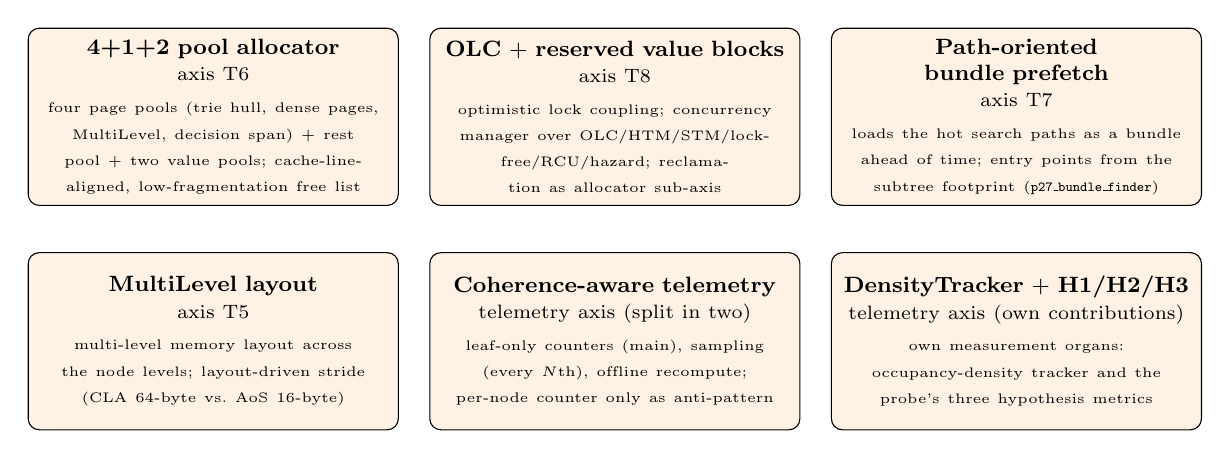
\begin{tikzpicture}[font=\footnotesize,
  pa/.style={draw,rounded corners,fill=orange!10,minimum width=4.7cm,minimum height=2.25cm,text width=4.4cm,align=center,inner sep=3pt}]
  \node[pa] (p1) at (0,0){\textbf{4+1+2 pool allocator}\\{\scriptsize axis T6}\\[2pt]{\tiny four page pools (trie hull, dense pages, MultiLevel, decision span) $+$ rest pool $+$ two value pools; cache-line-aligned, low-fragmentation free list}};
  \node[pa] (p2) at (5.1,0){\textbf{OLC $+$ reserved value blocks}\\{\scriptsize axis T8}\\[2pt]{\tiny optimistic lock coupling; concurrency manager over OLC/HTM/STM/lock-free/RCU/hazard; reclamation as allocator sub-axis}};
  \node[pa] (p3) at (10.2,0){\textbf{Path-oriented bundle prefetch}\\{\scriptsize axis T7}\\[2pt]{\tiny loads the hot search paths as a bundle ahead of time; entry points from the subtree footprint (\texttt{p27\_bundle\_finder})}};
  \node[pa] (p4) at (0,-2.85){\textbf{MultiLevel layout}\\{\scriptsize axis T5}\\[2pt]{\tiny multi-level memory layout across the node levels; layout-driven stride (CLA 64-byte vs.\ AoS 16-byte)}};
  \node[pa] (p5) at (5.1,-2.85){\textbf{Coherence-aware telemetry}\\{\scriptsize telemetry axis (split in two)}\\[2pt]{\tiny leaf-only counters (main), sampling (every $N$th), offline recompute; per-node counter only as anti-pattern}};
  \node[pa] (p6) at (10.2,-2.85){\textbf{DensityTracker $+$ H1/H2/H3}\\{\scriptsize telemetry axis (own contributions)}\\[2pt]{\tiny own measurement organs: occupancy-density tracker and the probe's three hypothesis metrics}};
\end{tikzpicture}
\caption{Gallery of the six own key points of PRT-ART, each at its axis: a 4+1+2 pool allocator (T6), optimistic lock coupling with reserved value blocks (T8), path-oriented bundle prefetch (T7), a MultiLevel layout (T5) and cache-coherence-aware telemetry together with the DensityTracker and the hypothesis metrics H1/H2/H3 --- the telemetry axis is split in two, a sweep sub-axis of the measurement tooling and a compile-time quantity of the builder (Section~\ref{sec:axis-triad}). The tiles show the \emph{building blocks of the probe repo}; overridden in the apparatus are the path-compression redirect (T3, engine-side reference composition), the prefetch (T7) and the ChainRef value handle (T10, slot composition of the probe) as well as the build axis page type; the building blocks for T5/T6 run in the measurement path via the cache-engine default, OLC is inherited from ART, and the remaining organ axes the slot composition draws from the ART reference of the cache engine (sixteen of eighteen).}\label{fig:prtart-gallery}
\end{figure}

\section{Axis Implementation and Measurement-System Levels}\label{sec:axes-impl}
Each axis is implemented as a generalized interface; alongside lie the levels of the measurement system
from code generation to the seven-phase pipeline. The section closes with the level picture E4--E0 in
code (Figure~\ref{fig:impl-layers}) and the contract surfaces at the carrier binaries; the register of
the design patterns used follows at the end of the chapter (Figure~\ref{fig:muster}).
Each axis is a topic directory that contains a two-layer \emph{concept}~\cite{sutton2012concepts} (a
broad topic concept and a narrow axis concept) as well as a \emph{CRTP base class} secured by a
\texttt{requires} clause. The live path of building-block selection is monomorphic: per axis, a
complete type list of all known building blocks (\texttt{All*}) is carried, from which a compile-time
filter over the enable flag of each building block (\texttt{mp\_filter<is\_enabled>},
Boost.Mp11~\cite{dimov_mp11}) forms the \texttt{Enabled*} list, and a composition assigns exactly one
type of this list per slot. The hot path contains neither \texttt{virtual} calls nor runtime switches
--- the zero-cost abstraction from Section~\ref{sec:anatomy-model}, in the sense of the C++ principle
that an unused abstraction costs nothing~\cite{stroustrup2012foundations}. Every SOTA design and every
allocator is integrated via a thin \emph{adapter} that provides the original implementation behind the
engine ABI\@: allocator vendors are attached via per-vendor include shims
(\texttt{\#if COMDARE\_AXIS\_06\_USE\_<X>} with forward stubs), where \texttt{USE} is the product of the
enable flag of the configuration and the detection flag \texttt{COMDARE\_HAVE\_<X>} of the build system
--- a missing vendor switches the building block off instead of breaking the build ---; SOTA building
blocks are switched on or off at compile time via constexpr enable flags together with
\texttt{mp\_filter} (the \texttt{COMDARE\_AXIS\_*\_USE\_}/\texttt{ENABLE\_} flag family), each with a
safe fallback chosen per family: allocator adapters replace the missing vendor in \texttt{if constexpr}
branches with the portable aligned allocation (\texttt{portable\_aligned\_alloc}), the vendor shim
supplies only forward stubs for the never-executed branch, and the axis value \texttt{StdMalloc} is a
building block of its own, not a makeshift; data-structure adapters of foreign search techniques
possess, behind their enable flag, a self-contained re-implementation as body, while the binding to the
original code runs via the library build with the original compiler --- a stub that throws an exception
at runtime does not occur in the organ axes (the types thrown there are contract violations such as
\texttt{invalid\_argument}, \texttt{length\_error} or \texttt{logic\_error} and the allocation errors
\texttt{bad\_alloc} and \texttt{bad\_array\_new\_length}, no \texttt{runtime\_error}) ---, so that the
build remains independently runnable. The organ axes not occupied by the probe draw their building
block from the cache engine by the same route (Section~\ref{sec:prtart-impl}). The integration of
hierarchical prefetching~\cite{zhang2025hierarchical} additionally provides a compile-time call-graph
analyser (\texttt{p27\_bundle\_finder}, a C++23 port of the original tool \texttt{hp\_soft} that
identifies functions with a subtree footprint above a threshold as bundle entry points).

A design decision delimits this live path from a rejected alternative: a variant-based building-block
resolution --- \texttt{resolve\_baustein} over \texttt{baustein\_variants}, a concept-checked
\texttt{if constexpr} over tag specializations --- is expressly forbidden for static organ axes because
it produces runtime overhead and code bloat; it exists only as a test cluster isolated from the build,
with one test as consumer of its resolution path (a second test reads from it only a building-block
identifier) and a strictness check that breaks any wiring into the codegen path. The reason is the
parsimony of the compiled artefact: a tier binary maps exactly the one permutation being run;
\texttt{std::variant}, \texttt{virtual} and runtime switches are forbidden in tier and hybrid binaries
because they map at runtime onto several compile-time targets --- whoever needs another permutation
needs another compiled artefact. The one permitted variant site of the house is the dock array of the
hybrid stage (\texttt{HybridDockVariant}, Section~\ref{sec:impl-hybrid-lager}), whose zone a test
checks by reading the source files and permitting exactly one occurrence; besides this, the code
tolerates \texttt{std::variant} in two axis-foreign building blocks (the error domain
\texttt{axis\_error} and the pressure state \texttt{pressure\_state}), which belong to no organ, and in
the three expected/result seams of the hardware probes (NUMA pages, NUMA core binding, operating
system) that consume the error sums of \texttt{axis\_error}; the CEB itself contains no variant site:
its substance under \texttt{builder/} lies within the counting range of the same check, and the one
registry header of its carrier scaffold under \texttt{libs/traeger/ceb} outside this range is likewise
variant-free. The ban is thus stricter than the mere avoidance of virtual
calls~\cite{alexandrescu2001modern}: it forbids every form of runtime branching between building
blocks.

Within each axis category there are main axes, sub-axes and meta-meta axes. In code, the category is
the trichotomy \texttt{AxisCategory} with the fixed order mess $<$ system $<$ organ --- an order that a
\texttt{static\_assert} holds against silent re-sorting ---, and the family of an axis is the
discriminator \texttt{AxisKind} with six values: measurement-system axis and measurement meta-meta,
system-configuration axis and system meta-meta, organ axis and organ meta-meta. A sub-axis is itself a
full axis (the recursion of the layer model remains open), and a sub-axis can at the same time be a
permutation axis --- the two roles do not exclude each other. Table~\ref{tab:axis-typology} counts the
inventory per category: the organ realm comprises eighteen main axes, twenty sub-axis headers and the
organ meta-meta \texttt{disk\_io}; the system realm three main axes, the complex axis
\texttt{build\_target\_complex} as command wrapper of their recombination with the sub-axis group
\texttt{build\_toolchain} (compiler, optimization level, atomics), the scheduling with five dimensions
and the system meta-metas under the hub of the extension hardware; the measurement realm the tooling
main axis (wallclock/macro/micro), four registered sub-axes (sixteen categories, work mode, measurement
framework, write-back method) and the measurement meta-meta \texttt{load\_framework}. The designation
meta-meta follows the four-level meta-level architecture of the Object Management Group
(MOF)~\cite{omg2016mof}, in which each level is the description language of the one beneath it; the
reading M0--M3 for this apparatus is developed in Section~\ref{sec:impl-system-axes}.
\begin{table}[htbp]\centering\footnotesize
\begin{tabular}{@{}lp{2.5cm}p{4.15cm}p{2.7cm}p{3.2cm}@{}}
\toprule
Category & Main axes & Sub-axes & Meta-meta axes & Single source \\
\midrule
Measurement & tooling (3: wallclock, macro, micro) & 16 categories; work mode (4); measurement framework (1); write-back method (4) & \texttt{load\_framework} (YCSB) & four registry headers, measurement registry XML \\
System & 3: \texttt{target\_\allowbreak{}isa}, \texttt{operating\_\allowbreak{}system}, \texttt{external\_\allowbreak{}utils} & complex axis \texttt{build\_target\_complex} with group \texttt{build\_toolchain} (3); \texttt{target\_isa\_complex} (3 members); scheduling (5 dimensions) & system meta-metas under the hub \texttt{external\_utils} & \texttt{kSystemAxisOrder}, system registry XML \\
Organ & 18 (T0--T17) & 20 sub-axis headers (e.g.\ SA1--SA4, AA1--AA7) & \texttt{disk\_io} (\texttt{binary\_id} $=$ \texttt{never}) & \texttt{kOrganAxisCount}, \texttt{kComposition\-AxisNames}, organ registry XML \\
\bottomrule
\end{tabular}
\caption{Axis typology per category (\texttt{AxisCategory} with the order mess $<$ system $<$ organ;
family discriminator \texttt{AxisKind} with six values). The numbers are structural numbers of the
source tree (registry headers and generated registry XML), not measured values.}\label{tab:axis-typology}
\end{table}

The eighteen organ axes (T0--T17, Section~\ref{sec:axis-triad}) are here not abstract but each a
concrete \emph{strategy concept} with several interchangeable building blocks, from which a concrete
composition chooses exactly one per slot; their number is, as \texttt{kOrganAxisCount} $=$ 18, the
single source of the organ line, and their names and slot order are carried by the array
\texttt{kCompositionAxisNames}. Figure~\ref{fig:axes-gallery} gathers all eighteen as a gallery --- per
axis the short name, the sub-axis family and a representative selection of the building blocks; the
complete building-block matrix with all origin sources is given in Appendix~\ref{app:blocks}, the SOTA
contributions per axis in Table~\ref{tab:axes-overview}.
Next to the eighteen canonical main axes stands the organ meta-meta \texttt{disk\_io}, which never
touches the \texttt{binary\_id} (Section~\ref{sec:axis-triad}); a nineteenth, optional organ axis is
planned but not implemented; only its implementation introduces it as slot T18.
That no composition omits an organ is enforced by the \texttt{IsComposition} concept: it demands per
algorithm the assignment of exactly these eighteen organs --- the fifteen search axes, the two queuing
axes and the persistence target ---, so that no composition compiles that leaves an axis open; the
complete organ set is
thus not a convention but a compile-time-checked condition.
\begin{figure}[htbp]\centering
% No \resizebox: the gallery is re-flowed from 5x4 to 4x5 tiles (~15.9cm instead of ~17.8cm wide,
% tiles 3.35->3.75cm, grid 4.05cm) and fits natively into \textwidth (16cm); this keeps the
% \footnotesize font unscaled instead of shrunk via resizebox (x0.90). Rule: resizebox only to
% SHRINK (cf. fig:m-model).
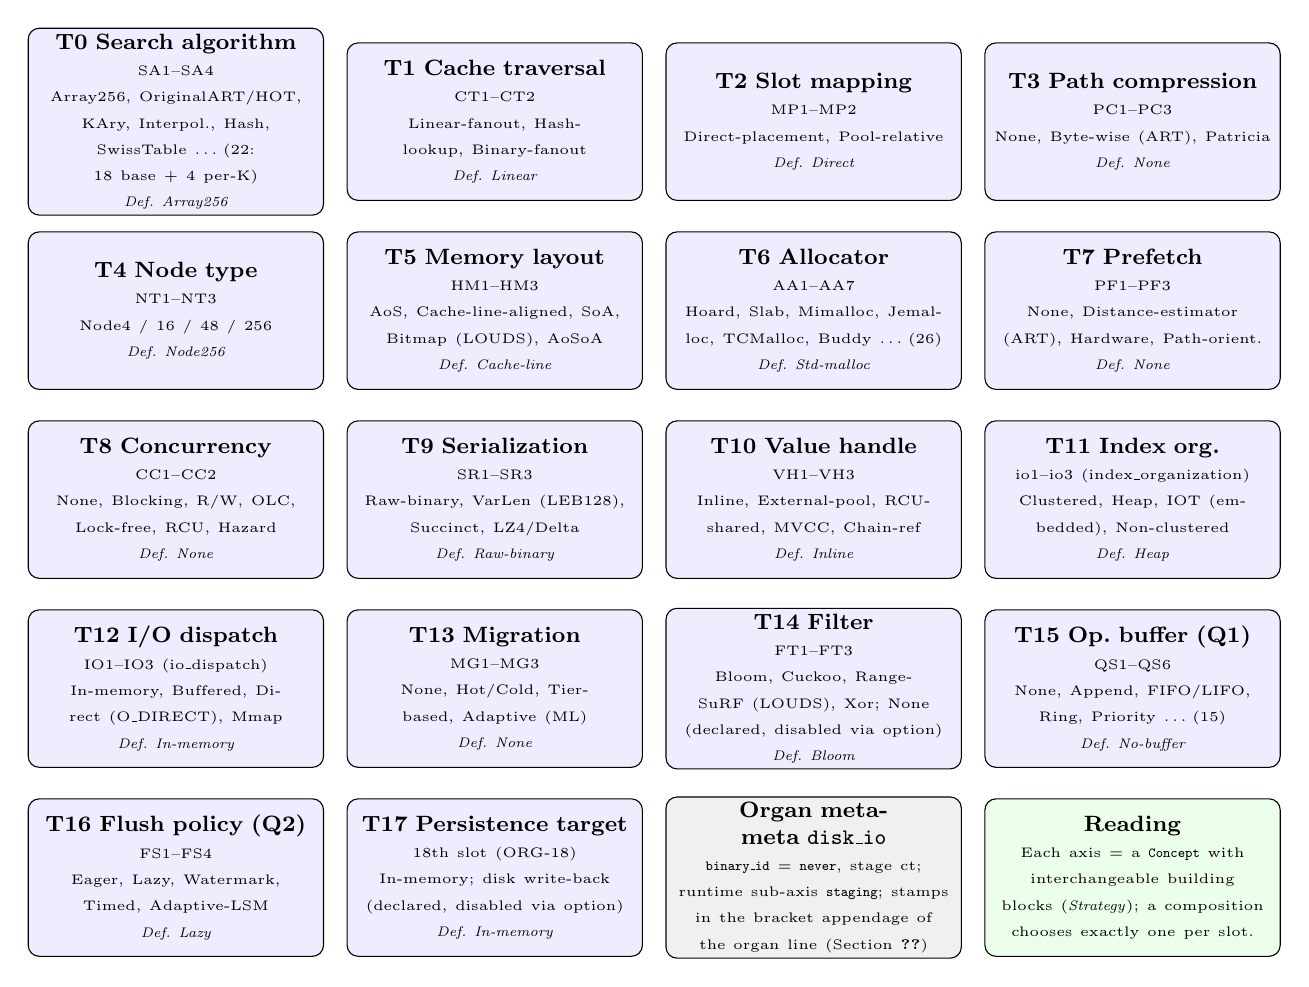
\begin{tikzpicture}[font=\footnotesize,
  ax/.style={draw,rounded corners,fill=blue!7,minimum width=3.75cm,minimum height=2.0cm,text width=3.55cm,align=center,inner sep=2pt}]
  \node[ax] (t0) at (0,0){\textbf{T0 Search algorithm}\\{\tiny SA1--SA4}\\{\tiny Array256, OriginalART/HOT, KAry, Interpol., Hash, SwissTable \dots\,(22: 18 base $+$ 4 per-K)}\\{\tiny\itshape Def.\ Array256}};
  \node[ax] (t1) at (4.05,0){\textbf{T1 Cache traversal}\\{\tiny CT1--CT2}\\{\tiny Linear-fanout, Hash-lookup, Binary-fanout}\\{\tiny\itshape Def.\ Linear}};
  \node[ax] (t2) at (8.1,0){\textbf{T2 Slot mapping}\\{\tiny MP1--MP2}\\{\tiny Direct-placement, Pool-relative}\\{\tiny\itshape Def.\ Direct}};
  \node[ax] (t3) at (12.15,0){\textbf{T3 Path compression}\\{\tiny PC1--PC3}\\{\tiny None, Byte-wise (ART), Patricia}\\{\tiny\itshape Def.\ None}};
  \node[ax] (t4) at (0,-2.4){\textbf{T4 Node type}\\{\tiny NT1--NT3}\\{\tiny Node4 / 16 / 48 / 256}\\{\tiny\itshape Def.\ Node256}};
  \node[ax] (t5) at (4.05,-2.4){\textbf{T5 Memory layout}\\{\tiny HM1--HM3}\\{\tiny AoS, Cache-line-aligned, SoA, Bitmap (LOUDS), AoSoA}\\{\tiny\itshape Def.\ Cache-line}};
  \node[ax] (t6) at (8.1,-2.4){\textbf{T6 Allocator}\\{\tiny AA1--AA7}\\{\tiny Hoard, Slab, Mimalloc, Jemalloc, TCMalloc, Buddy \dots\,(26)}\\{\tiny\itshape Def.\ Std-malloc}};
  \node[ax] (t7) at (12.15,-2.4){\textbf{T7 Prefetch}\\{\tiny PF1--PF3}\\{\tiny None, Distance-estimator (ART), Hardware, Path-orient.}\\{\tiny\itshape Def.\ None}};
  \node[ax] (t8) at (0,-4.8){\textbf{T8 Concurrency}\\{\tiny CC1--CC2}\\{\tiny None, Blocking, R/W, OLC, Lock-free, RCU, Hazard}\\{\tiny\itshape Def.\ None}};
  \node[ax] (t9) at (4.05,-4.8){\textbf{T9 Serialization}\\{\tiny SR1--SR3}\\{\tiny Raw-binary, VarLen (LEB128), Succinct, LZ4/Delta}\\{\tiny\itshape Def.\ Raw-binary}};
  \node[ax] (t10) at (8.1,-4.8){\textbf{T10 Value handle}\\{\tiny VH1--VH3}\\{\tiny Inline, External-pool, RCU-shared, MVCC, Chain-ref}\\{\tiny\itshape Def.\ Inline}};
  \node[ax] (t11) at (12.15,-4.8){\textbf{T11 Index org.}\\{\tiny io1--io3 (index\_organization)}\\{\tiny Clustered, Heap, IOT (embedded), Non-clustered}\\{\tiny\itshape Def.\ Heap}};
  \node[ax] (t12) at (0,-7.2){\textbf{T12 I/O dispatch}\\{\tiny IO1--IO3 (io\_dispatch)}\\{\tiny In-memory, Buffered, Direct (O\_DIRECT), Mmap}\\{\tiny\itshape Def.\ In-memory}};
  \node[ax] (t13) at (4.05,-7.2){\textbf{T13 Migration}\\{\tiny MG1--MG3}\\{\tiny None, Hot/Cold, Tier-based, Adaptive (ML)}\\{\tiny\itshape Def.\ None}};
  \node[ax] (t14) at (8.1,-7.2){\textbf{T14 Filter}\\{\tiny FT1--FT3}\\{\tiny Bloom, Cuckoo, Range-SuRF (LOUDS), Xor; None (declared, disabled via option)}\\{\tiny\itshape Def.\ Bloom}};
  \node[ax] (t15) at (12.15,-7.2){\textbf{T15 Op.\ buffer (Q1)}\\{\tiny QS1--QS6}\\{\tiny None, Append, FIFO/LIFO, Ring, Priority \dots\,(15)}\\{\tiny\itshape Def.\ No-buffer}};
  \node[ax] (t16) at (0,-9.6){\textbf{T16 Flush policy (Q2)}\\{\tiny FS1--FS4}\\{\tiny Eager, Lazy, Watermark, Timed, Adaptive-LSM}\\{\tiny\itshape Def.\ Lazy}};
  \node[ax] (t17) at (4.05,-9.6){\textbf{T17 Persistence target}\\{\tiny 18th slot (ORG-18)}\\{\tiny In-memory; disk write-back (declared, disabled via option)}\\{\tiny\itshape Def.\ In-memory}};
  \node[draw,rounded corners,fill=gray!12,minimum width=3.75cm,minimum height=2.0cm,text width=3.55cm,align=center,inner sep=2pt] (mm) at (8.1,-9.6){\textbf{Organ meta-meta \texttt{disk\_io}}\\{\tiny \texttt{binary\_id} $=$ \texttt{never}, stage ct; runtime sub-axis \texttt{staging}; stamps in the bracket appendage of the organ line (Section~\ref{sec:axis-triad})}};
  \node[draw,rounded corners,fill=green!8,minimum width=3.75cm,minimum height=2.0cm,text width=3.55cm,align=center,inner sep=2pt] (leg) at (12.15,-9.6){\textbf{Reading}\\{\tiny Each axis $=$ a \texttt{Concept} with interchangeable building blocks (\emph{Strategy}); a composition chooses exactly one per slot.}};
\end{tikzpicture}
\caption{Gallery of the eighteen organ axes (T0--T17, canonical slot order): per axis the implementation concept --- short name, sub-axis family and a representative selection of the interchangeable building blocks. Each axis is a \texttt{Concept} interface with several strategy building blocks (\emph{Strategy} pattern); a concrete composition occupies exactly one per slot. The \emph{default} (\enquote{Def.}) is a derived comparison baseline, not a code flag. The numbers in parentheses (T0, T6, T15) are the \emph{catalogues} of the complete type lists (\texttt{All*}); the \emph{enabled inventory} of a build configuration is the subset formed by the enable filter, which the generated registry XML reports per axis (for instance four search algorithms and three allocators in the in-house default). The T numbers are slots of the composition, not directory numbers of the implementation; the abbreviations io1--io3 and IO1--IO3 belong to different axes (index organization and I/O dispatch). Next to the eighteen slots stands the organ meta-meta \texttt{disk\_io}; the persistence target is pinned to its in-memory representative in the canonical reference catalogue (Section~\ref{sec:axis-triad}). The complete matrix with origin sources is given in Appendix~\ref{app:blocks}.}\label{fig:axes-gallery}
\end{figure}

\subsection{The One Architecture in Code}\label{sec:impl-architecture}
The \emph{one} architecture from Section~\ref{sec:anatomy-model} is, in code, a single hierarchy.
Its root is \texttt{IExecutionEngine} with three engine kinds --- Anatomy, Virus, Hybrid --- and a
contract of seven methods: \texttt{warm\_up}, \texttt{run}, \texttt{reset} and \texttt{shutdown} as
measurement lifecycle as well as \texttt{engine\_name}, \texttt{engine\_kind} and
\texttt{lifecycle\_state} as reports. Beneath it lie, on level~1, the four families Map, Container,
Graph and HeuristikAdapter (Section~\ref{sec:anatomy-levels}) --- Graph as a declared stub without a
genus --- and, on level~2, the six genera SearchAlgorithm, Set, Sequence, Adapter, View and
FunctionInterfaceReroute; in code the family is the derivation of the genus (\texttt{gattung\_of}), not
a second label. The living being \texttt{SearchAlgorithm} and its ABI runtime view --- the
\enquote{SearchEngine} --- are two views of the same entity across the module boundary, not a parallel
construct: the body is \texttt{SearchAlgorithmAnatomy<C>}, the composition and wiring of the eighteen
organs, and the view is \texttt{SearchAlgorithmAbiAdapter<A>}, which exports it across the module
boundary. The layering \texttt{CacheEngine}\,$\to$\,\texttt{ExecutionEngine}\,$\to$\,\texttt{SearchEngine}
(cf.\ Section~\ref{sec:repos}) thus separates roles, not class trees: the \texttt{CacheEngine} as the
axis building-block library, the \texttt{ExecutionEngine} as the living root of the execution and
measurement tools (OS primitives; in experiment mode the measurement aggregator over exactly one
observer interface) and the \texttt{SearchEngine} as the search-API view measured over precisely this
interface --- the library skeleton of the same name, \texttt{libs/search\_engine}, contains no code
(Section~\ref{sec:repos}). Axis-less \emph{viruses} stand as siblings beneath the same root (in the
existing code a graph breadth-first search) but possess no anatomy (Figure~\ref{fig:one-architecture}).
In this hierarchy the compiler-compiler character of the apparatus is anchored: every composition is a
type from which the builder generates a separate compiled artefact per permutation.

\begin{figure}[!htbp]
  \centering
  % No \resizebox: the drawing is only ~15.5cm wide and fits natively into \textwidth (16cm); the former
  % \resizebox{0.95\textwidth} (x0.98) merely scaled the \footnotesize font against the body text.
  % Rule: resizebox only to SHRINK genuine overwidth (cf. fig:m-model).
  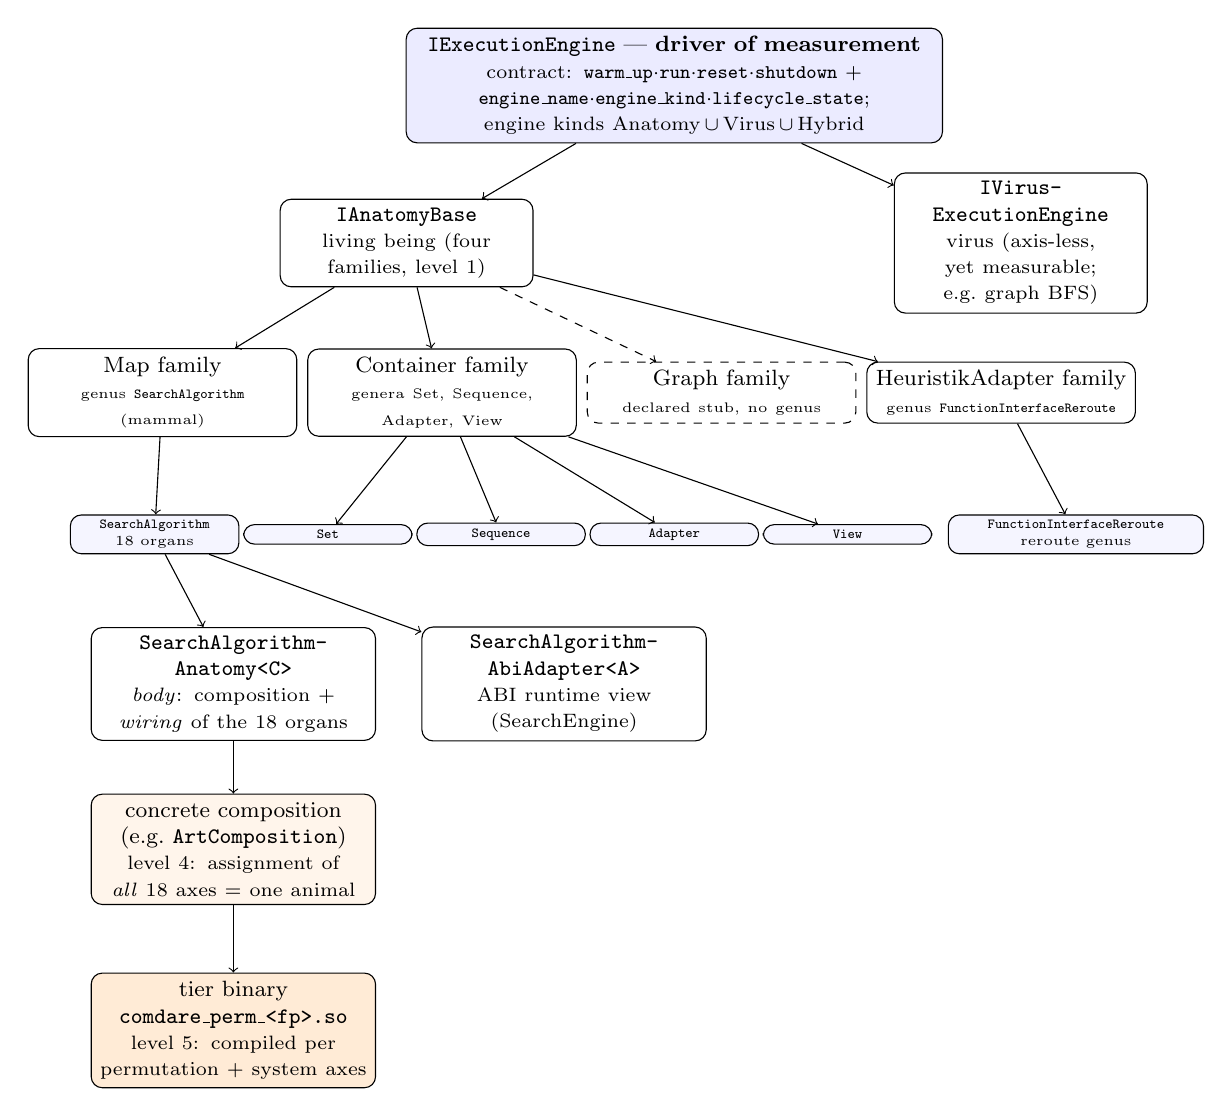
\begin{tikzpicture}[box/.style={draw, rounded corners, align=center, font=\footnotesize, inner sep=3pt, text width=3.0cm},
    gen/.style={draw, rounded corners, align=center, font=\tiny, inner sep=2pt, text width=2.0cm, fill=blue!4}]
    \node[box,fill=blue!8,text width=6.6cm] (root) at (-1.0,0) {\texttt{IExecutionEngine} --- \textbf{driver of measurement}\\{\scriptsize contract: \texttt{warm\_up$\cdot$run$\cdot$reset$\cdot$shutdown} $+$ \texttt{engine\_name$\cdot$engine\_kind$\cdot$lifecycle\_state}; engine kinds Anatomy\,$\cup$\,Virus\,$\cup$\,Hybrid}};
    \node[box] (ana) at (-4.4,-2.0) {\texttt{IAnatomyBase}\\{\scriptsize living being (four families, level~1)}};
    \node[box] (vir) at (3.4,-2.0) {\texttt{IVirus\-Execution\-Engine}\\{\scriptsize virus (axis-less, yet measurable; e.g.\ graph BFS)}};
    \node[box,text width=3.2cm] (g1) at (-7.5,-3.9) {Map family\\{\tiny genus \texttt{SearchAlgorithm} (mammal)}};
    \node[box,text width=3.2cm] (g2) at (-3.95,-3.9) {Container family\\{\tiny genera Set, Sequence, Adapter, View}};
    \node[box,text width=3.2cm,dashed] (g3) at (-0.4,-3.9) {Graph family\\{\tiny declared stub, no genus}};
    \node[box,text width=3.2cm] (g4) at (3.15,-3.9) {HeuristikAdapter family\\{\tiny genus \texttt{FunctionInterfaceReroute}}};
    \node[gen] (n1) at (-7.6,-5.7) {\texttt{SearchAlgorithm}\\18 organs};
    \node[gen] (n2) at (-5.4,-5.7) {\texttt{Set}};
    \node[gen] (n3) at (-3.2,-5.7) {\texttt{Sequence}};
    \node[gen] (n4) at (-1.0,-5.7) {\texttt{Adapter}};
    \node[gen] (n5) at (1.2,-5.7) {\texttt{View}};
    \node[gen,text width=3.1cm] (n6) at (4.1,-5.7) {\texttt{FunctionInterfaceReroute}\\reroute genus};
    \node[box,text width=3.4cm] (body) at (-6.6,-7.6) {\texttt{Search\-Algorithm\-Anatomy<C>}\\{\scriptsize \emph{body}: composition $+$ \emph{wiring} of the 18 organs}};
    \node[box,text width=3.4cm] (abi) at (-2.4,-7.6) {\texttt{Search\-Algorithm\-Abi\-Adapter<A>}\\{\scriptsize ABI runtime view (\enquote{SearchEngine})}};
    \node[box,fill=orange!8,text width=3.4cm] (comp) at (-6.6,-9.7) {concrete composition (e.g.\ \texttt{ArtComposition})\\{\scriptsize level 4: assignment of \emph{all} 18 axes $=$ one animal}};
    \node[box,fill=orange!16,text width=3.4cm] (bin) at (-6.6,-12.0) {tier binary \texttt{comdare\_perm\_\-<fp>.so}\\{\scriptsize level 5: compiled per permutation $+$ system axes}};
    \draw[->] (root) -- (ana);
    \draw[->] (root) -- (vir);
    \draw[->] (ana) -- (g1); \draw[->] (ana) -- (g2); \draw[->,dashed] (ana) -- (g3); \draw[->] (ana) -- (g4);
    \draw[->] (g1) -- (n1);
    \draw[->] (g2) -- (n2); \draw[->] (g2) -- (n3); \draw[->] (g2) -- (n4); \draw[->] (g2) -- (n5);
    \draw[->] (g4) -- (n6);
    \draw[->] (n1) -- (body);
    \draw[->] (n1) -- (abi);
    \draw[->] (body) -- (comp);
    \draw[->] (comp) -- (bin);
  \end{tikzpicture}
  \caption{The \emph{one} architecture as a single hierarchy without parallel trees. At the root stands
  \texttt{IExecutionEngine} as the \emph{driver of measurement} --- the universal measurable contract of
  measurement lifecycle (\texttt{warm\_up}/\texttt{run}/\texttt{reset}/\texttt{shutdown}) and reports
  (\texttt{engine\_name}/\texttt{engine\_kind}/\texttt{lifecycle\_state}) across all three engine kinds
  Anatomy, Virus and Hybrid; beneath it branch the anatomy-bearing \emph{families} (level~1: Map,
  Container, Graph, HeuristikAdapter) with their \emph{genera} (level~2) and the axis-less
  \emph{viruses}. \texttt{SearchAlgorithm} \emph{is} the focal living being (mammal); its anatomy is its
  \emph{body} --- the fixed composition \emph{and wiring} of the 18 organs ---, and
  \enquote{SearchEngine} only its ABI runtime view. The mammal branch is drawn out down to the
  individual: a concrete axis composition (level~4) is compiled per permutation as a standalone tier
  binary (level~5). Container possesses an organ set of its own with the genera Set, Sequence, Adapter
  and View, whose arities are carried by the genus build admission; Graph is declared and possesses no
  genus; the family HeuristikAdapter carries the reroute genus of the hybrid stage.}\label{fig:one-architecture}
\end{figure}

Concretely, the module boundary is a C-stable interface --- the ABI (application binary interface) of
the apparatus --- that exports exactly one living being per permutation (Figure~\ref{fig:abi}): every
tier binary contains seven mandatory symbols with C linkage --- the four primal symbols ABI version,
magic number, factory \texttt{comdare\_\allowbreak{}create\_\allowbreak{}anatomy} and destroy, plus the
two reports \texttt{comdare\_\allowbreak{}anatomy\_\allowbreak{}gattung} and
\texttt{comdare\_\allowbreak{}anatomy\_\allowbreak{}genus}, spelled identically across all families, as
well as the version lines of the stamp. The identical spelling is a condition, not a convenience: the
family-independent loader loads every binary via the same loading route (POSIX
\texttt{dlopen}~\cite{posix_dlopen}) and can determine the family \emph{before} it constructs an
instance --- family-independent names with family-specific values; the family is here derived from the
genus. The ABI carries major version~9, whose seam is the genus interface. The variadic 1/2/N hybrid
API belongs to the probe: its \texttt{PrtArtSearchEngine<Ts\ldots>} specializes by parameter count ---
one parameter demands all function interfaces of a \texttt{std::vector}, two those of a
\texttt{std::map}, more than two those of a \texttt{std::map} onto a tuple ---, and the slot arities of
the genera of the cache engine (eighteen for the genus SearchAlgorithm, each their own for Set,
Sequence, Adapter and View from the genus build admission) are to be read separately from it. Complex
keys are reduced by a fingerprint component of the cache engine
(\texttt{fixed\_\allowbreak{}length\_\allowbreak{}fingerprint}, FNV-1a base) to 16-byte binary strings
of fixed length, which the probe uses as the key type of its memory model (\texttt{BinaryKey}); this key
fingerprint is to be distinguished from the three identity fingerprints of the apparatus --- the 64-bit
field \texttt{permutation\_\allowbreak{}fingerprint} in the ABI POD of the module, the SHA-512 tier
fingerprint (format~6, eleven members) and the SHA-256 planner fingerprint
(Section~\ref{sec:stamp-model}). How these and the remaining code interfaces relate in detail is
summarized by the UML map in Figure~\ref{fig:uml-interfaces}.

\begin{figure}[!htbp]
\begin{lstlisting}[basicstyle=\footnotesize\ttfamily,frame=single,xleftmargin=1.5em]
// C-stable module boundary: seven mandatory symbols per tier binary
extern "C" {
  std::uint64_t comdare_anatomy_abi_version();   // ABI major 9
  std::uint64_t comdare_anatomy_abi_magic();     // compatibility probe
  IAnatomyBase* comdare_create_anatomy();        // one being per permutation
  void          comdare_destroy_anatomy(IAnatomyBase*);
  std::uint8_t  comdare_anatomy_gattung();       // same name for every family
  std::uint8_t  comdare_anatomy_genus();         // hybrid: the target genus
  AnatomyVersionLines const* comdare_anatomy_version_lines();
}
// The hybrid .so exports the same set: exactly one loading route.

// Probe view: variadic 1/2/N API (key K, values V)
//   1 parameter  ->  std::vector<V>
//   2 parameters ->  std::map<K, V>
//   N > 2        ->  std::map<K, std::tuple<V1, ..., VN>>
template<class K, class First, class... Rest> class PrtArtSearchEngine;
\end{lstlisting}
  \caption{The ABI-stable C module boundary (seven mandatory symbols; the hybrid \texttt{.so} exports the same set
  and reports its target genus via \texttt{genus}) and the variadic 1/2/N API as the view of the probe.
  Complex keys are reduced by a fingerprint component to 16-byte binary strings of fixed length; the
  identity of a binary is carried separately from this by the \texttt{permutation\_fingerprint} field of
  the ABI POD, the SHA-512 tier fingerprint and the SHA-256 planner fingerprint.}\label{fig:abi}
\end{figure}

\begin{figure}[htbp]\centering
% No \resizebox: the drawing is only ~15.3cm wide; blowing it up to 0.96\linewidth (x1.006) would inflate
% the \scriptsize font beyond the body text. Rule: resizebox only to SHRINK (cf. fig:m-model).
\begin{tikzpicture}[font=\footnotesize,>=Stealth,align=center,
  iface/.style={draw,rounded corners,fill=blue!7,minimum width=4.6cm,minimum height=0.72cm,font=\ttfamily\scriptsize},
  comp/.style={draw,fill=green!8,minimum width=4.6cm,minimum height=0.72cm,font=\ttfamily\scriptsize},
  alt/.style={draw,dashed,gray,minimum width=4.6cm,minimum height=0.72cm,font=\ttfamily\scriptsize,text=gray}]
  \node[font=\bfseries\scriptsize] at (-4.9,5.8){Engine/anatomy hierarchy};
  \node[iface,minimum height=1.0cm] (exec) at (-4.9,5.05){IExecutionEngine\\{\normalfont\scriptsize driver of measurement}};
  \node[iface] (anat) at (-4.9,3.75){IAnatomyBase};
  \node[iface] (virus) at (-0.2,5.05){IVirusExecutionEngine};
  \node[comp] (gatt) at (-4.9,2.75){Family (4, level 1)};
  \node[comp] (genus) at (-4.9,1.75){Genus (6, level 2)};
  \node[comp] (body) at (-4.9,0.75){SearchAlgorithmAnatomy<C>};
  \node[comp] (abi) at (-4.9,-0.25){SearchAlgorithmAbiAdapter<A>};
  \node[iface,fill=orange!10] (drive) at (-4.9,-1.35){IDriveableTier / IObservableTier};
  \node[iface,fill=orange!10] (mess) at (-4.9,-2.35){IMessVisitor\\{\normalfont\scriptsize surface 3: measurement cut-through}};
  \draw[->] (exec)--(anat); \draw[->] (exec.east) to[bend left=10] (virus.west);
  \draw[->] (anat)--(gatt); \draw[->] (gatt)--(genus); \draw[->] (genus)--(body); \draw[->] (body)--(abi); \draw[->] (abi)--(drive); \draw[->] (drive)--(mess);
  \node[font=\bfseries\scriptsize] at (4.9,5.8){Implementation pattern per axis ($\times$18)};
  \node[iface] (topic) at (4.9,5.05){TopicConcept $\wedge$ AxisConcept};
  \node[comp] (crtp) at (4.9,3.95){AxisBase<Derived> (CRTP)};
  \node[comp] (all) at (4.9,2.85){All*: mp\_list<Baustein$_{1..k}$>};
  \node[comp] (filt) at (4.9,1.75){mp\_filter<is\_enabled>};
  \node[comp] (en) at (4.9,0.65){Enabled* list};
  \node[iface] (slot) at (4.9,-0.45){Composition slot (exactly one type)};
  \node[alt] (resolve) at (4.9,-1.75){resolve\_baustein<Tag> (rejected)};
  \draw[->] (topic)--(crtp); \draw[->] (crtp)--(all); \draw[->] (all)--(filt); \draw[->] (filt)--(en); \draw[->] (en)--(slot);
  \draw[->,dashed,gray] (body.east) to[bend right=14] node[midway,below,font=\scriptsize\itshape,text=gray]{composes 18 axes} (topic.west);
\end{tikzpicture}
\caption{UML map of the code interfaces: on the left the engine/anatomy hierarchy --- the measurable root \texttt{IExecutionEngine} as the \emph{driver of measurement} (Anatomy\,$\cup$\,Virus\,$\cup$\,Hybrid) over \texttt{IAnatomyBase}, the four families and six genera and the axis-less \texttt{IVirus\-Execution\-Engine}, beneath it the \emph{body} \texttt{Search\-Algorithm\-Anatomy<C>} (composition \emph{and wiring} of the eighteen axes) and its ABI runtime view \texttt{Search\-Algorithm\-Abi\-Adapter<A>} (\enquote{SearchEngine}), which is measured via the drive/observer contracts \texttt{IDriveableTier}/\texttt{IObservableTier} and whose measurement crosses as surface~3 through the visitor \texttt{IMessVisitor}; on the right the live path repeated per axis --- a two-layer \texttt{Concept}, a \texttt{requires}-secured CRTP base, the complete \texttt{mp\_list} building-block family, the compile-time filter over the enable flag and the composition slot, which contains exactly one type. The variant-based resolution \texttt{resolve\_baustein} is a rejected alternative isolated from the build (dashed).}\label{fig:uml-interfaces}
\end{figure}

\subsection{From Profile to Tier Binary: Planner, Builder and Measurement Pipeline}\label{sec:impl-pipeline}
The chain from the user XML to the tier binary (Section~\ref{sec:mess-chain}) has, in code, a named
shape of two binaries. Stage~1, the planner role, is \texttt{comdare-experiment-planner} with the
subcommands \texttt{validate}, \texttt{plan dump|ci|cmake}, \texttt{cache-key}, \texttt{fingerprint},
\texttt{status}, \texttt{check-size}, \texttt{simulate}, \texttt{version} and \texttt{help}.
\texttt{validate} checks, purely read-only, the profile resolved by the XML parser against the
compiled-in registry catalogues (an unregistered reference is a hard validation error,
Section~\ref{sec:mess-chain}), builds no binary in doing so and does not measure. \texttt{plan} drives
the deterministic walk of the \texttt{ExperimentPlanDirector} --- separated along the design patterns
\emph{Director} and \emph{Builder}~\cite{gamma1994patterns}: the director owns the \emph{one}
enumeration walk over measurement combinations, system permutations and organ steps, and per output
syntax (text plan, CI pipeline description, CMake fragment) a concrete builder emits via hook methods
---; two runs are byte-identical, and the plan header annotates the registry trio of the three offering
catalogues organ/system/measurement. \texttt{check-size} and \texttt{simulate} compute the measurement
set before the run from the inputs of the walk (Section~\ref{sec:impl-contracts}). Stage~2, the CEB
role, is the measurement driver \texttt{comdare-messung-driver} in the project repository with the
subcommands \texttt{tier ci|cmake}, \texttt{run}, \texttt{version} and \texttt{help}: it emits the view
of the second chain stage --- system permutations and tier build orders of its released build space ---
and drives the measurement run; a planner topic addressed to it is answered by its dispatcher with the
reference to the planner binary instead of silently executing it. The planner steers the CEB orders,
the CEB steers the tier orders: the separation of roles is thus not merely surface but two modules. The
emitted build and check attestations keep the layer separation of the chain visible --- their legends
have three forms: \texttt{ceb:build:[a,b,c]} on stage~1; on stage~2 per host a build and check batch
\texttt{tier:build-batch:<host>}, whose attestations per step contain the separate system and organ
brackets \texttt{zelle=[d,e,f][g,h,i]} and which bundles the organ build volumes internally into slices
of 4096 binaries each (the milestone batches in Section~\ref{sec:fairness}); and per host a measurement
batch \texttt{measure:[a,b,c]:batch:<host>}, whose measurement attestations alone contain all three
brackets \texttt{zelle=[a,b,c][d,e,f][g,h,i]} (Figure~\ref{fig:traeger-stufen}); the brackets name only
main axes, sub-axes are pure runtime permutation and appear in no build legend.

The installation has two control paths: the planner directly via shell, and an API command line with a
headless service that serves the planner as a cell on Kubernetes or on bare metal, so that a complete
measurement series can be triggered and observed without an interactive session. Added to this is a
command-line-guided creation mode for the user XML with hardware filter: options not available on the
target machine are not selectable in it, and the mode is optional --- a hand-written XML remains
equivalent. Present in the code are the planner's hardware probe, which queries the host at runtime,
and the three machine signatures of the system registry; implementation status: the shell path is
implemented; service and creation mode are planned but not implemented.

Two properties secure the \emph{one} main channel. First, the text plan (format v1.1) reports per build
step the actually generated file stem (\texttt{built\_stem}) --- produced by the \emph{same}
orchestrator function that the build orchestrator also calls during the build: the plan claims no name
that the build does not produce, and a stem that cannot be determined is written as \enquote{-} instead
of synthesized. Second, there is \emph{one} XML source and \emph{one} channel that builds it: variant
formation lies in the C++23 metaprogramming, CMake is confined to the role of building, and a second
emission channel for permutation source texts does not exist in the source tree.

Inside the CEB, the builder transforms each profile into a precompiled C++23 module. Each permutation
is identified by a bit-packed \emph{permutation flag} structure that comprises ten banks of 64~bits
each (page type, node, traversal, value handle, layout, allocator, prefetch, concurrency, ISA and
telemetry) and is serialized hexadecimally; the allocator sub-axes AA1--AA7 carry a flag bank of their
own. A constraint filter of the flag structure (\texttt{is\_valid\_combination}, four rules, for
instance: leaf-only counters only together with retroactive aggregation) excludes incoherent
combinations. The measurement path identifies the eighteen organ axes via the string-serialized
eighteen-segment path (the \texttt{binary\_id}, Section~\ref{sec:stamp-model}) together with the three
fingerprints; the permutation count over the axes follows a mixed-radix encoding in which each axis is
a digit with its own base --- the shape of a product space as described by the variability models of
software product lines~\cite{pohl2005spl}. Over these building blocks runs the
\emph{seven-phase measurement pipeline} (Figure~\ref{fig:pipeline}) of the \texttt{ExperimentDriver}
library per series with the phases of the code: (1)~\textsc{Enumerate} (parse XML configs, build the
permutation list), (2)~\textsc{Generate} (one \texttt{comdare\_perm\_<fp>.cpp} per permutation plus
aggregator CMakeLists, in addition
\texttt{generate\_\allowbreak{}module\_\allowbreak{}from\_\allowbreak{}profile} for the SOTA profiles),
(3)~\textsc{Compile} (CMake configuration and build of all permutation modules),
(4)~\textsc{Link+Load} (\texttt{dlopen} of all modules), (5)~\textsc{Execute} (\texttt{create\_instance}
+ profile-aware \texttt{run\_workload}), (6)~\textsc{Measure} (aggregate binary measurement records)
and (7)~\textsc{Persist} (CSV and JSON, optionally binary); two opt-in phases compile missing modules
in the running experiment (\texttt{phase3\_hot\_compile\_missing}) and run a functional test per module
--- creating and destroying an instance, a \texttt{run\_workload} with an empty workload descriptor and
the check of the ABI version (\texttt{phase4b\_functional\_tests}). The measurement-series modes
\texttt{Defined}, \texttt{Full} and \texttt{FullSampled} (deterministic 1:$n$ subset of the full space,
Section~\ref{sec:mess-chain}) choose which permutations a series comprises. The downstream evaluation
toolchain (Figure~\ref{fig:toolchain}) is a sequence of nine numbered programs from
\texttt{sample\_data\_generator} to \texttt{tex\_formatter}; its output is the xlsx workbook, the
standard; the CSV form is not a single child document but an ordered tree of CSV files --- one overall
folder per workbook, beneath it one folder per sheet, therein the CSV files of the individual sub-axis
runs ---, which is always generated from the workbook (xlsx to csv, as a strategy of the same factory)
and, per XML, lies at the same target instead of the workbook or in addition to it (four registered
write-back methods, Section~\ref{sec:impl-system-axes}). Implementation status: the seam writes the CSV
projection as one flat file (\texttt{projektion\_\allowbreak{}oeffnen} in
\texttt{ergebnis\_\allowbreak{}mappe\_\allowbreak{}naht}); the tree form is planned but not implemented.
The measurement couplings are separated from the production path by the
\texttt{COMDARE\_\allowbreak{}MEASUREMENT\_\allowbreak{}ON} gating (Section~\ref{sec:repos}), and
continuous integration~\cite{fowler2006ci} runs across all four repositories (GitLab CI\@; the
repositories are additionally mirrored to GitHub).
\begin{figure}[htbp]\centering
% No \resizebox: the drawing is only ~13.5cm wide; blowing it up to \linewidth (x1.19) would inflate
% the \footnotesize font beyond the body text. Rule: resizebox only to SHRINK (cf. fig:m-model).
\begin{tikzpicture}[font=\footnotesize,>=Stealth,align=center,
  ph/.style={draw,rounded corners,fill=blue!6,minimum width=1.6cm,minimum height=0.85cm},
  hi/.style={draw,rounded corners,fill=orange!18,very thick,minimum width=1.6cm,minimum height=0.85cm},
  opt/.style={draw,rounded corners,dashed,fill=orange!8,minimum width=2.0cm,minimum height=0.65cm,font=\scriptsize},
  pb/.style={draw,rounded corners,fill=orange!16,very thick,minimum width=3.7cm,minimum height=1.05cm,text width=3.5cm,font=\scriptsize}]
  \node[font=\bfseries\scriptsize,anchor=west] at (-0.95,0.95){In-process path --- \texttt{ExperimentDriver} (7 phases)};
  \node[ph] (p1) at (0,0){\textbf{1}\\Enumerate};
  \node[ph] (p2) at (1.95,0){\textbf{2}\\Generate};
  \node[hi] (p3) at (3.9,0){\textbf{3}\\Compile};
  \node[ph] (p4) at (5.85,0){\textbf{4}\\Link+Load};
  \node[hi] (p5) at (7.8,0){\textbf{5}\\Execute};
  \node[hi] (p6) at (9.75,0){\textbf{6}\\Measure};
  \node[ph] (p7) at (11.7,0){\textbf{7}\\Persist};
  \foreach \a/\b in {p1/p2,p2/p3,p3/p4,p4/p5,p5/p6,p6/p7}{\draw[->,thick] (\a)--(\b);}
  \node[font=\scriptsize,text=orange!60!black] at (3.9,0.66){\textsc{Build}};
  \node[font=\scriptsize,text=orange!60!black] at (8.78,0.66){\textsc{Measure}};
  \node[opt] (o1) at (2.9,-1.4){opt-in:\\hot-compile};
  \node[opt] (o2) at (5.4,-1.4){opt-in:\\functional test per module};
  \draw[->,dashed] (o1)--(p3);
  \draw[->,dashed] (o2)--(p4);
  \node[font=\bfseries\scriptsize,anchor=west] at (-0.95,-2.5){Out-of-process path --- \texttt{BuildOrchestrator} $+$ \texttt{perm\_runner} (design decision)};
  \node[pb] (b1) at (2.0,-3.95){\textbf{build} \texttt{Build\-Orchestrator}: builds \emph{all} tier binaries first (resumable, RAM-aware)};
  \node[pb] (b2) at (8.0,-3.95){\textbf{measure} \texttt{perm\_runner}: loads $+$ measures each tier binary individually (1 DLL/process, via \texttt{IObservableTier})};
  \draw[->,very thick] (b1)--node[above,font=\scriptsize]{tier binaries} (b2);
\end{tikzpicture}
\caption{The measurement pipeline in two forms. The \textbf{in-process path} (top) is the seven-phase
pipeline of the \texttt{ExperimentDriver} per measurement series (Enumerate $\to$ Generate $\to$ Compile
$\to$ Link+Load $\to$ Execute $\to$ Measure $\to$ Persist; two opt-in phases compile missing modules in
the running experiment and run a functional test per module with ABI version check). Highlighted are the
substantial phases: \textsc{Compile} (the \emph{build} of the tier binaries) and
\textsc{Execute}/\textsc{Measure} (the \emph{measurement}); Generate/Link+Load/Persist are wiring. The
\textbf{out-of-process path} (bottom) is a design decision for process isolation: the
\texttt{BuildOrchestrator} \emph{first} builds \emph{all} tier binaries (resumable, RAM-aware), after
which \texttt{perm\_runner} loads and measures each binary individually via the observer interface
\texttt{IObservableTier} --- one DLL per process, because the DLL contains no \texttt{main} and the
runner is the executable that loads it; no state is shared between permutations, and a cluster task
runs exactly one runner with exactly one DLL.}\label{fig:pipeline}
\end{figure}
\begin{figure}[htbp]\centering
% No \resizebox: the chain is deliberately broken into three rows (~12.1cm wide),
% so the font stays unscaled. Rule: resizebox only to SHRINK (cf. fig:m-model).
\begin{tikzpicture}[font=\footnotesize,>=Stealth,align=center,
  tool/.style={draw,rounded corners,fill=blue!6,minimum height=0.7cm,minimum width=3.4cm,inner sep=5pt,font=\ttfamily\scriptsize}]
  \node[tool] (t1) at (0,0){01 sample\_data\_generator};
  \node[tool] (t2) at (4.35,0){02 messung\_driver};
  \node[tool] (t3) at (8.7,0){03 binary\_to\_csv};
  \node[tool] (t4) at (0,-1.5){04 csv\_to\_latex};
  \node[tool] (t5) at (4.35,-1.5){05 diagram\_generator};
  \node[tool] (t6) at (8.7,-1.5){06 latex\_to\_pdf};
  \node[tool] (t7) at (0,-3.0){07 tier\_binary\_report};
  \node[tool] (t8) at (4.35,-3.0){08 appendix\_generator};
  \node[tool] (t9) at (8.7,-3.0){09 tex\_formatter};
  \draw[->,thick] (t1)--(t2);
  \draw[->,thick] (t2)--(t3);
  \draw[->,thick] (t3.south) -- ++(0,-0.4) -- ([yshift=0.4cm]t4.north) -- (t4.north);
  \draw[->,thick] (t4)--(t5);
  \draw[->,thick] (t5)--(t6);
  \draw[->,thick] (t6.south) -- ++(0,-0.4) -- ([yshift=0.4cm]t7.north) -- (t7.north);
  \draw[->,thick] (t7)--(t8);
  \draw[->,thick] (t8)--(t9);
\end{tikzpicture}
\caption[The downstream evaluation toolchain]{The downstream evaluation toolchain as a nine-stage
chain: \texttt{sample\_data\_generator} produces deterministic test data without real hardware,
\texttt{messung\_driver} drives the measurement series (the CEB role), \texttt{binary\_to\_csv}
deserializes the binary measurement records, \texttt{csv\_to\_latex} renders the booktabs tables with a
building-block fact sheet per permutation ID and produces no file on empty input,
\texttt{diagram\_generator} the A4-aware TikZ diagrams (three basic plot types bar, scatter and heatmap
as well as the families of the measurement appendix built on them: ECDF staircase, range bars, stacked
per-axis attribution, sweep curve, 3D raw-data view, ratio matrix, normalized bars, Pareto scatter and
the observer detail table), \texttt{latex\_to\_pdf}
typesets the manuscript, \texttt{tier\_binary\_report} rasters per tier binary the interface contract
against the planned set of the text plan, \texttt{appendix\_generator} generates, as an in-process
facade per language, the core and presentation files of the measurement appendix from \emph{one} WIDE
matrix, and \texttt{tex\_formatter} normalizes the generated files. The output of the chain is the xlsx
workbook; the CSV form is not a single child document but the ordered tree of CSV files generated from
the workbook (one folder per sheet), written in code as one flat file (the tree form is planned but not
implemented; Section~\ref{sec:impl-system-axes}).}\label{fig:toolchain}
\end{figure}

The levels E4--E0 from Section~\ref{sec:anatomy-layers} each have a place in code, and the boundaries
between them each have a contract test (Section~\ref{sec:impl-contracts});
Figure~\ref{fig:impl-layers} shows this code shape without explaining the levels anew. E4, the
definition and evaluation layer, is the XML profile with the planner
(\texttt{profile\_\allowbreak{}facade/\allowbreak{}planner}) and the evaluation programs 04 and 08 of
the toolchain; E3, the permutation B\textsuperscript{+}-tree, is the experiment tree
(\texttt{experiment\_tree}) with the \texttt{binary\_id} as path; E2, the tier binaries, is the ABI
adapter with the module ABI declaration; E1, the runtime configuration, is the interface
\texttt{IResourceControllableTier} together with the dynamic dimensions of the measurement registry
XML\@; E0, the infrastructure, is CI, runners and store; the cross-cutting concern~M is the
system-axis root \texttt{SystemAxis} (Section~\ref{sec:impl-system-axes}).
\begin{figure}[htbp]\centering
\begin{tikzpicture}[font=\footnotesize,>=Stealth,
  eb/.style={draw,rounded corners,fill=blue!7,minimum width=11.4cm,minimum height=0.95cm,text width=11.1cm,align=left,inner sep=3pt},
  ct/.style={font=\tiny,fill=white,inner sep=1pt}]
  \node[eb] (e4) at (0,0){\textbf{E4} definition/evaluation layer --- {\scriptsize XML profile $+$ planner (\texttt{profile\_facade/planner}); evaluation: programs 04 and 08}};
  \node[eb] (e3) at (0,-1.55){\textbf{E3} permutation B$^+$-tree --- {\scriptsize \texttt{experiment\_tree}; path $=$ \texttt{binary\_id} (18 segments, mixed-radix)}};
  \node[eb] (e2) at (0,-3.1){\textbf{E2} tier binaries --- {\scriptsize \texttt{SearchAlgorithmAbiAdapter<A>} $+$ module ABI declaration (seven mandatory symbols)}};
  \node[eb] (e1) at (0,-4.65){\textbf{E1} runtime configuration --- {\scriptsize \texttt{IResourceControllableTier} $+$ dynamic dimensions of the measurement registry XML}};
  \node[eb,fill=gray!12] (e0) at (0,-6.2){\textbf{E0} infrastructure --- {\scriptsize CI (four repositories), runners, store}};
  \draw[->,thick] (e4)--(e3); \draw[->,thick] (e3)--(e2); \draw[->,thick] (e2)--(e1); \draw[->,thick] (e1)--(e0);
  \node[ct] at (0,-0.775){\texttt{test\_e4\_contract\_xml\_to\_axislevels} (fake E3)};
  \node[ct] at (0,-2.325){\texttt{test\_e3\_contract\_binary\_id\_bijektion} $+$ \texttt{\ldots\_conformance\_gate\_wirksam} (fake E2)};
  \node[ct] at (0,-3.875){\texttt{test\_e2\_contract\_abi\_vertrag} (Wormhole reference DLL, fake E1)};
  \node[ct] at (0,-5.425){\texttt{test\_e1\_contract\_rc\_konsum} (in-process, T6/T8/T1/T11)};
  \node[draw,rounded corners,fill=orange!12,minimum width=2.8cm,minimum height=7.15cm,text width=2.6cm,align=center,inner sep=3pt] (m) at (7.3,-3.1){\textbf{M} measurement cross-cutting concern\\[3pt]{\scriptsize \texttt{SystemAxis} root, host-side; touches no binary identity}\\[3pt]{\tiny \texttt{test\_m\_\allowbreak contract\_\allowbreak system\_\allowbreak axis\_\allowbreak wurzel}, \texttt{test\_b3\_\allowbreak wallclock\_\allowbreak erbe\_ct}}};
\end{tikzpicture}
\caption[The levels E4--E0 in code]{The levels E4--E0 of the layer model (Section~\ref{sec:anatomy-layers}) at their place in code,
with the contract test per boundary (fake of the neighbouring level) and the measurement cross-cutting
concern~M, which crosses all levels host-side without touching the binary identity.}\label{fig:impl-layers}
\end{figure}

The contracts between the carrier stages are partitioned into surfaces at the binaries. The
three-surface model (Section~\ref{sec:anatomy-levels}) is present in code by name: surface~1 is the
genus interface of the tier binary (runtime, abstract factory), surface~2 the stamp (compile time,
ABI-stable) and surface~3 the measurement cut-through \texttt{IMessVisitor} --- a visitor at the
\texttt{dlopen} transition with double dispatch, which exists \emph{so that} family and genus interfaces
remain unchanged: the measurement crosses as a seam of its own instead of forcing measurement fields
into the domain interfaces. The stamp contract is executed as a matrix of seven interfaces and four
carriers --- 28~cells with three-valued admission (mandatory, permitted, forbidden), of which the existing
code occupies only mandatory and forbidden (Table~\ref{tab:stempel-matrix}): the static self-version is
carried only by the planner; measurement and system line are carried by CEB, tier and hybrid; the organ
line is carried only by tier and hybrid --- the absence at the CEB is the static barrier \enquote{the CEB
carries no organ axes} ---; fingerprint and overall stamp are carried by all four, and the attached
stamp lines are carried only by the hybrid as runtime hook. The contract is checked not in the base but
beneath every heir: the base is empty, and only a
\texttt{static\_assert(StempelVertrag<Erbin, Traeger>)} directly beneath the definition turns an
unparsable line, a missing mandatory or a forbidden interface into a compilation error --- a form of
consumer-driven contract~\cite{robinson2006cdc}, in which the expectation of the consuming carrier
drives the contract.
\begin{table}[htbp]\centering\footnotesize
\begin{tabular}{@{}llcccc@{}}
\toprule
Interface & Content & Planner & CEB & Tier & Hybrid \\
\midrule
\texttt{VersionXyz}     & static self-version X.Y.Z[.flag]                  & M & F & F & F \\
\texttt{MessZeile}      & stamp line of the measurement realm               & F & M & M & M \\
\texttt{SystemZeile}    & stamp line of the system realm                    & F & M & M & M \\
\texttt{OrganZeile}     & stamp line of the organ realm                     & F & F & M & M \\
\texttt{FingerprintSha} & fingerprint hex (planner SHA-256, otherwise SHA-512) & M & M & M & M \\
\texttt{GesamtStempel}  & the one composite of the heir                     & M & M & M & M \\
\texttt{Angeschlossene} & attached stamp lines (runtime hook)               & F & F & F & M \\
\bottomrule
\end{tabular}
\caption{The stamp contract as a matrix of seven interfaces and four carriers (28 cells, three-valued
admission M = mandatory, P = permitted, F = forbidden; P is unoccupied in the existing code). The
forbidden cell of the organ line at the CEB is the static barrier \enquote{the CEB carries no organ axes};
the cells are checked per heir via \texttt{static\_assert}.}\label{tab:stempel-matrix}
\end{table}

\section{Quality Assurance: Contract Tests per Layer}\label{sec:impl-contracts}
The layer model E4--E0 with its fixed interface contracts was developed as a concept in
Section~\ref{sec:anatomy-layers}; this section describes its implementation as test infrastructure.
The reason lies in the layering itself: changes that alter several layers at once produce errors from
interactions between the levels that neither local tests nor line-by-line review make visible (ADR-5,
Appendix~\ref{app:adr}). For a system whose product space rules out any complete materialization
(Section~\ref{sec:mess-chain}), changes across several levels at once are thus practically not
acceptable; the consequence is to complete each layer individually --- with an explicitly fixed
interface contract to the neighbouring level, its own test harness and its own definition of
acceptance.

The carrying test principle reads: \emph{each layer is tested against a compile-time substitute of its
neighbouring level.} The contract tests are ordinary test targets of the build pipeline; the
neighbouring level is replaced in each case by a \emph{fake} --- a template- and concept-based stand-in
in the test scope, no runtime switch in production code. A layer can thus be finished and accepted
before the deeper level even consumes its values, and the test question of every boundary --- does the
layer pass its definition on to the next one \emph{without loss}?
(Section~\ref{sec:anatomy-layers}) --- turns from a design principle into an executable acceptance
test.

Per layer this takes concrete shape as follows (Figure~\ref{fig:impl-layers}): for the definition and
evaluation layer~E4 the harness
(\texttt{test\_\allowbreak{}e4\_\allowbreak{}contract\_\allowbreak{}xml\_\allowbreak{}to\_\allowbreak{}axislevels})
checks the translation of the declarative XML profiles into the axis-level structure --- golden
fixtures compare the axis levels emitted from a profile structurally against an expected reference,
with a fake E3 replacing the permutation tree; neither tree construction nor build orders are needed to
accept the boundary E4$\to$E3. For the permutation B\textsuperscript{+}-tree~E3 the harness
(\texttt{test\_\allowbreak{}e3\_\allowbreak{}contract\_\allowbreak{}binary\_\allowbreak{}id\_\allowbreak{}bijektion})
checks the bijection of the binary identity: from axis-level fixtures the permutation enumeration is
run and, per path, the mixed-radix-encoded binary identifier is translated back and forth (counting
plus signature round trip) --- against a fake E2 that builds not a single binary; added to this is a
conformance gate in the full-run path
(\texttt{test\_\allowbreak{}e3\_\allowbreak{}contract\_\allowbreak{}conformance\_\allowbreak{}gate\_\allowbreak{}wirksam}),
which checks every imported binary against the fixed contract before the measurement. For the tier
binaries~E2 the contract is the ABI itself
(\texttt{test\_\allowbreak{}e2\_\allowbreak{}contract\_\allowbreak{}abi\_\allowbreak{}vertrag}): the
Wormhole reference DLL is loaded and must satisfy the fixed interface sequence ---
\texttt{IAnatomyBase}, \texttt{IObservableTier} and \texttt{IResourceControllableTier} (present at every
adapter) together with a fixed capability report. The response to a control-quantity request
(\texttt{apply}) is here not an error code but the \emph{number of axes that actually accepted the
value}: a request above the reported capabilities becomes visible because this number stays below the
number of requested axes --- in the Wormhole pilot, of five controllable axes exactly two (batch size
and inline threshold) actually accept the value, a null pointer yields zero ---, and that is the
completeness rule of the control quantities: nothing is accepted silently, every response counts only
the real consumption. The accompanying fake E1 creates the runtime control quantities and applies them,
but demands no consumption effect --- that belongs to the acceptance of E1. For the runtime
configuration~E1, finally, edge tests
(\texttt{test\_\allowbreak{}e1\_\allowbreak{}contract\_\allowbreak{}rc\_\allowbreak{}konsum}, in-process
over the axes T6, T8, T1 and T11) check the corner cases of the dynamic regime: that a reused tier is
completely reset between two runs, that a pool budget below the live data set is treated as a named
state instead of silently violated and that every applied control quantity is visible as a named column
in the persisted result file, plus the preservation of the two-phase operation loop (discarded warm-up,
measurement run) as an invariant.
Persistence is checked at the result file, not at the in-process state; the lead here is the standard
xlsx --- the write-back registry carries it as the fourth method and default evaluation format, the
xlsx writer lies in the storage layer of the store ---, and the CSV form is not a single child document
but an ordered tree of CSV files (one overall folder per workbook, beneath it one folder per sheet,
therein the CSV files of the individual sub-axis runs), which is always generated from the workbook
and, per XML, lies at the same target instead of the workbook or in addition to it. Implementation
status: the E1 check reads the CSV output of the persist phase, which the seam writes as one flat file
(\texttt{projektion\_\allowbreak{}oeffnen}); the check at the xlsx generated per binary and the tree
form of the CSV storage are planned but not implemented.

Above the layer harnesses, a \emph{two-gate protocol} secures every implementation package. Its
purpose is the separation of two questions: gate~1 secures the engine repository against itself --- the
unit and contract tests ---, gate~2 secures the integration into the project repository, in which the
chain XML $\to$ binaries $\to$ measurement $\to$ appendix actually runs; only both together prove that
a package does not break the apparatus (continuous integration and delivery as safeguarding
stages~\cite{fowler2006ci,humble2010cd}).
\emph{Gate~1} is the strict gate of the engine repository: the full test suite\footnote{Extent of the
  test suite: 551 registered tests (\texttt{ctest -N}) in the gcc release build tree of
  17~September 2026.} runs in four cells, gcc and clang each as release and debug build, without change
skip, and only a run without failed tests is accepted, without an exception list. The double run has
two reasons: the compiler matrix forces every static check through two translators, and the repetition
of the measurement run --- the two-phase operation loop of discarded warm-up and measurement run in the
single-thread-deterministic mode \texttt{measure} --- makes the run-to-run stability of the number
itself the object of testing. Part of gate~1 is the golden anchoring of the permutation space, and here
two notions are to be separated (Section~\ref{sec:mess-chain}):
The \emph{reference catalogue} of the golden test holds $2^{17} = 131072$ binary identities ---
seventeen axes with two representatives each, the persistence target pinned to one --- and is confirmed
against a fixed CRC-64 checksum (\texttt{0x56F1B721C72DC10E}, CRC-64/ECMA-182 over the identities in % chktex 29
canonical order; the reference is literal tool output, and its change is permissible only within a
coordinated interface change), while a small, materializable catalogue of
$4\cdot4\cdot5\cdot4 = 320$ identities serves as a byte-exact check of the serialization form --- a
characterization test in the sense of Feathers~\cite{feathers2004legacy}, which uses a fixed
cardinality as a regression detector. The \emph{cardinality} of the space planned in a complete
measurement series is different from this and never static: the planner counts it per axis from the
possibilities declared in the XML in the director walk (\texttt{check-size}, \texttt{simulate}) and
multiplies the levels over all axes; it differs per platform through missing releases, and every number
of the computation comes in as input, never as a constant.
\emph{Gate~2} is the integration gate of the project repository: its pipeline builds without error and
without an exception set --- the rule of this work knows no tolerated failing tests; the two declared
failure tolerances of the measurement machines lie in the engine repository and are a platform boundary
(an arm64 smoke build without an available runner) and a manual relock maintenance job (it must not
remain in the executed state), not a test set.

This protocol is methodology, not a system component: it describes \emph{how} changes to the apparatus
are accepted, not what the binaries contain. The directory and suite structure on which it runs is
documented in Appendix~\ref{app:code}.

Completion follows the layering top-down --- E4, E3, E2, then the measurement cross-cutting concern~M
immediately before E1 ---, and the infrastructure~E0 forms the last step of the consolidation
(Section~\ref{sec:anatomy-layers}). The degree of maturity can be read from the test inventory: all
four boundaries possess their harness (above), and the cross-cutting concern~M possesses one of its own
that gets by without any tier binary
(\texttt{test\_\allowbreak{}m\_\allowbreak{}contract\_\allowbreak{}system\_\allowbreak{}axis\_\allowbreak{}wurzel}
for the system-axis root and the measurement visitability,
\texttt{test\_\allowbreak{}b3\_\allowbreak{}wallclock\_\allowbreak{}erbe\_\allowbreak{}ct} for the
wallclock inheritance): a synthetic measurement source is driven through the system-axis root and its
values traced into the result columns. The measurement axis here drives the release of the measurement
source via the system-axis root in the shape of the CEB\@: the planner delegates to the CEB interface
which binary recombination is to be measured against which loads, and the CEB releases the source.
Implementation status: the hardware acquisition chain runs at the release seam of the builder
(Section~\ref{sec:impl-system-axes}); the CEB-driven release path of the measurement source is planned
but not implemented. The code shape of the cross-cutting concern is described in the following section.

\section{Realm Roots in Code: System and Measurement Axes}\label{sec:impl-system-axes}
Four abstraction levels order the notions of this section (Figure~\ref{fig:m0-m3}), following the
four-level meta-level architecture of the Object Management Group (MOF)~\cite{omg2016mof}, in which M0
denotes the runtime instances, M1 the model, M2 the metamodel and M3 the meta-metamodel: M3 are the
\emph{meta-meta axes} in the sense of the indirection of a description --- an axis that describes how
other axes are described (the measurement meta-meta \texttt{load\_framework}, the organ meta-meta
\texttt{disk\_io}, the system meta-metas under the hub of the extension hardware); M2 are, as a
reading, the \emph{meta axes}, the literal classification of the main and sub-axes carried under their
notion --- in code the registry line with category, family and building-block list; M1 are conception
and runtime implementation of the main and sub-axes --- the CRTP axis with its concept; M0 is the
binary code --- the tier binary in which exactly one assignment is compiled in. In the stamp, the
meta-meta level of an entry is mechanically its bracket depth: bits~3--5 of an entry encode the level,
a main axis is bracket-less, a meta-meta hangs as a bracket appendage on its line, and a depth above
seven aborts with an error message; the renderer of the meta-meta entries is at the same time the
bottleneck at which two version checks check every stamped member, so that no new meta-meta can bypass
this check. The short form \texttt{c\{p.e\}} of a version flag here denotes \texttt{c} with the
sub-members \texttt{p} and \texttt{e}, never a flat abbreviation. Per realm there is a dedicated
meta-meta discriminator (\texttt{measurement\_meta\_meta}, \texttt{system\_meta\_meta},
\texttt{organ\_meta\_meta}); PMC acquisition --- performance monitoring counters, the hardware counters
of the CPU --- is a meta-meta measurement axis because it describes with which counter instrument other
measurements are collected.
\begin{figure}[htbp]\centering
\begin{tikzpicture}[font=\footnotesize,>=Stealth,
  mb/.style={draw,rounded corners,minimum width=13.6cm,minimum height=1.05cm,text width=13.3cm,align=left,inner sep=3pt}]
  \node[mb,fill=orange!14] (m3) at (0,0){\textbf{M3 meta-meta axes} --- indirection of a description\\{\scriptsize examples: \texttt{load\_framework} (measurement realm, token \texttt{ycsb@1.0.0.c}), \texttt{disk\_io} (organ realm, bracket appendage), system meta-metas under \texttt{external\_utils}}};
  \node[mb,fill=orange!8] (m2) at (0,-1.5){\textbf{M2 meta axes} (reading) --- literal classification of the main and sub-axes\\{\scriptsize example: the registry line \texttt{<axis id=allocator slot=T06 category=composition \ldots>} with its building-block list}};
  \node[mb,fill=blue!7] (m1) at (0,-3.0){\textbf{M1 conception and runtime implementation} --- main and sub-axes\\{\scriptsize example: the CRTP axis \texttt{AxisBase<Derived>} with its concept and its building blocks (Strategy)}};
  \node[mb,fill=gray!12] (m0) at (0,-4.5){\textbf{M0 binary code} --- the tier binary\\{\scriptsize example: \texttt{comdare\_perm\_<fp>.so} with exactly one compiled-in assignment; identity \texttt{binary\_id} $+$ fingerprint}};
  \draw[->,thick] (m3)--node[right,font=\tiny]{describes}(m2);
  \draw[->,thick] (m2)--node[right,font=\tiny]{classifies}(m1);
  \draw[->,thick] (m1)--node[right,font=\tiny]{compiles to}(m0);
\end{tikzpicture}
\caption[The four abstraction levels M0--M3]{The four abstraction levels M0--M3 as a reading of the axis notions, following the meta-level
architecture of the MOF\@: meta-meta axes (M3) describe how other axes are described; the registry
line (M2) classifies main and sub-axes; the CRTP axis (M1) is their conception and runtime
implementation; the tier binary (M0) is the binary code of exactly one assignment.}\label{fig:m0-m3}
\end{figure}

The tripartition of the axis realms (Section~\ref{sec:axis-triad}) is executed in code as a type
separation. All axes share a common family roof --- \texttt{topics::Axis<Derived>}, an empty,
non-polymorphic CRTP base whose concept check (\texttt{is\_empty} and not \texttt{is\_polymorphic})
rejects any smuggled-in vtable already at compile time --- and declare their category via the
trichotomy \texttt{AxisCategory} and their family via the discriminator \texttt{AxisKind} with six
values (Section~\ref{sec:axes-impl}). Per family there is a dedicated CRTP root: \texttt{OrganAxis}
and \texttt{OrganMetaMetaAxis} for the organ realm, \texttt{SystemAxis} for the measurement-system
axes of the host-side cross-cutting concern, \texttt{CebSystemAxis} for the build and steering axes of
the CEB configuration, \texttt{SystemMetaMetaAxis} for the system meta axes under the extension hub and
\texttt{MeasurementMetaMetaAxis} for the measurement-realm axes of the planner. An axis \emph{is} its
family through its base class, not through a re-attachable label --- \texttt{CebSystemAxis} returns
its kind \texttt{axis\_kind()} as the hard return value \texttt{system\_config}, which is why the
measurement realm possesses a root of its own instead of a reused one: the system realm roots at the
CEB, the measurement realm at the planner (Section~\ref{sec:axis-triad}).

On the system side, the canonical order itself is code: the system main axes \texttt{target\_isa},
\texttt{operating\_system} and \texttt{external\_utils} are held in their binding sequence by the
constant three-element array \texttt{kSystemAxisOrder}, and every consumer that needs an order --- the
stamp line, the generator block sequence, the XML header, the suffix segments --- must read it there
instead of re-deriving it (order single source with drift checks). Three compile-time \emph{re-entry
guards} fix the cut of the main axes: \texttt{static\_assert} checks reject compiler, scheduling and
load framework as system main axes --- the compiler is a sub-axis group \texttt{build\_toolchain} of
the complex wrapper \texttt{build\_target\_complex} with a global optimization identity in the
toolchain member of the fingerprint, the scheduling a sub-axis at \texttt{target\_isa} with five
dimensions, the load framework a meta-meta main axis of the measurement realm ---, and whoever
re-enters one of the three breaks the build and must revoke the assignment explicitly instead of
silently revising it. The build version identifier of the system line (Section~\ref{sec:stamp-model})
likewise draws from a single declarative source: the ordered eight-segment sequence
\texttt{kSuffixSegmentOrder} of the build control quantities --- compiler identifier, optimization,
SIMD extension, CEB, target ISA, telemetry, build type and gate contribution ---, in which an empty
member produces no segment and the gate segment stands at the end, so that every suffix comparison
sees an unchanged beginning and an appendage (prefix stability); the four-part cell path of the storage
follows the same order member by member, with a check that binds both orders to each other.

On the measurement side, the meta-meta root \texttt{MeasurementMetaMetaAxis} is the planner's own;
its first carrier is the load framework \texttt{load\_framework} (stamp token
\texttt{ycsb@1.0.0.c}), and like all measurement-realm axes it is strictly binary-id-neutral
(registry XML\@: \texttt{binary\_id} $=$ \texttt{never}). The measurement-tooling
\emph{main} axis holds exactly three versioned entries --- wallclock, macro, micro --- in the only
permitted order wallclock/macro/micro (alias w/ma/mi, Section~\ref{sec:measurement-system}); its check
turns a fourth, unagreed tooling into a compilation error. It fans out four sub-axis registries, one
file each (Table~\ref{tab:mess-registries}): the work mode (\texttt{WorkMode}: build, measure, compare,
release, Section~\ref{sec:repos}), the measurement framework (\texttt{MeasurementFramework}: exactly
one entry, YCSB), the write-back method (\texttt{WritebackMethod}: CSV, LaTeX table, comparison metrics
and xlsx --- four values, xlsx as default evaluation format, expressly no PDF, because the PDF
compilation is not a write-back channel of the measurement machine) and the sixteen measurement
categories (below); each registry is a \texttt{constexpr} catalogue with the static check index $=$
enum value, and a further entry breaks the compilation. The counter instrumentation resides in the
micro tooling; a PMC vendor registry supplements it with the hardware form of the counters (below). On
the compile side, two separate gates mirror this tooling ladder: the \emph{statistics gate}
(\texttt{COMDARE\_\allowbreak{}CE\_\allowbreak{}ENABLE\_\allowbreak{}STATISTICS}, an \texttt{\#ifdef})
switches the observer statistics of the macro regime, the value-based \emph{segment-timing gate}
(\texttt{COMDARE\_\allowbreak{}CE\_\allowbreak{}ENABLE\_\allowbreak{}SEGMENT\_\allowbreak{}TIMING}, an
\texttt{\#if}) the eighteen per-axis segment timers of the fine grain. An unset segment-timing gate
\emph{inherits} the state of the statistics gate --- existing builds do not change a single byte
through the separation ---, and a set segment-timing gate without the statistics gate aborts the
compilation with an error message, because the segment timers write into structures of the observer
block. The actually effective gate state of every translation unit travels as a dedicated
measurement-gate member with nine \texttt{;}-separated fields into the fingerprint preimage of the
stamp (Section~\ref{sec:stamp-model}) --- in the off state
\texttt{mg=m0;s0;st0;x0;tw0;tm0;tmi0;hm0;hmi0}: measurement, statistics, segment timing, experiment
mode, then wallclock, macro and micro of the tier stage and macro and micro of the hybrid stage on
positions of their own ---; the stamp thus never claims an outfit that the build does not carry. The
target picture next to this registry state is the axis-interface model from
Section~\ref{sec:mess-chain}: micro-benchmarking measures an axis via its axis interface, and the three
measurement levels provide the counter-measurement; the registry is aligned to this model.
\begin{table}[htbp]\centering\footnotesize
\begin{tabular}{@{}p{3.0cm}p{4.6cm}cp{4.0cm}@{}}
\toprule
Registry (file) & Values & Count & Check \\
\midrule
\texttt{run\_\allowbreak{}methodology\_\allowbreak{}registry} & \texttt{WorkMode}: build, measure, compare, release & 4 & index $=$ enum, execution order; only measure measures \\
\texttt{measurement\_\allowbreak{}framework\_\allowbreak{}registry} & \texttt{MeasurementFramework}: Ycsb & 1 & a second framework breaks at compile time \\
\texttt{writeback\_\allowbreak{}method\_\allowbreak{}registry} & \texttt{WritebackMethod}: Csv, LatexTable, ComparisonMetrics, Xlsx (default) & 4 & a fifth method breaks at compile time; no PDF \\
\texttt{measurement\_\allowbreak{}axis\_\allowbreak{}registry} & sixteen measurement categories with regime (9 time/observer, 7 PMC) & 16 & index $=$ category, no empty name, regime $=$ root assignment \\
\bottomrule
\end{tabular}
\caption{The four sub-axis registries of the measurement tooling: one \texttt{constexpr} file each with
index-equals-enum check; the main axis itself holds the three toolings wallclock, macro and
micro.}\label{tab:mess-registries}
\end{table}

Switching off the measurement is a staged model over the three measurement levels
(Figure~\ref{fig:abschaltungsstufen}). The measuring instrument \texttt{checkpoint\_measure} always
collects the input parameters at a \emph{point in time}; the first layer, the wallclock, is the minimum
of a time-measuring, otherwise parameter-empty checkpoint and thus the minimal measuring instrument of
the CEB\@. If macro or micro benchmarking is active, the wallclock checkpoint also performs the
parameter bracket --- a compile-time special case, because in macro and micro, parameters and time
measurement always coincide. The first shut-off level switches off the parameter collection in macro
and micro, so that the wallclock remains in place for \texttt{measure} and \texttt{compare}; the
second, permutative shut-off level lets the wallclock fall away as well for \texttt{release}, and with
it the surfaces and interfaces of the measurement fall away: for the release only the core code of the
binary remains standing. Implementation status: the code contains the gates G2 and G3 and the release
mode without instrumentation (\texttt{measurement\_on} off); the two-level shut-off as a permutation
quantity is planned but not implemented.
\begin{figure}[htbp]\centering
\begin{tikzpicture}[font=\footnotesize,>=Stealth,
  ze/.style={draw,rounded corners,minimum width=3.9cm,minimum height=1.35cm,text width=3.7cm,align=center,inner sep=2pt,font=\scriptsize},
  rl/.style={font=\scriptsize\bfseries,anchor=east,text width=2.6cm,align=right}]
  \node[font=\bfseries\scriptsize] at (0,1.2){wallclock (w)};
  \node[font=\bfseries\scriptsize] at (4.3,1.2){macro (ma)};
  \node[font=\bfseries\scriptsize] at (8.6,1.2){micro (mi)};
  \node[rl] at (-2.3,0){Stage 0: full measurement\\(\texttt{measure})};
  \node[ze,fill=orange!14] at (0,0){point in time $+$ parameter bracket (compile-time special case)};
  \node[ze,fill=orange!14] at (4.3,0){time $+$ parameters per genus-interface function};
  \node[ze,fill=orange!14] at (8.6,0){time $+$ success parameters per axis interface};
  \node[rl] at (-2.3,-1.7){Stage 1: parameters off\\(\texttt{measure}, \texttt{compare})};
  \node[ze,fill=orange!8] at (0,-1.7){point in time only: parameter-empty \texttt{checkpoint\_measure} (minimum)};
  \node[ze,fill=gray!10] at (4.3,-1.7){parameter collection switched off};
  \node[ze,fill=gray!10] at (8.6,-1.7){parameter collection switched off};
  \node[rl] at (-2.3,-3.4){Stage 2: everything off\\(\texttt{release})};
  \node[ze,fill=gray!18] at (0,-3.4){falls away --- no measurement surface, no measurement interface};
  \node[ze,fill=gray!18] at (4.3,-3.4){falls away};
  \node[ze,fill=gray!18] at (8.6,-3.4){falls away: only the core code of the binary};
\end{tikzpicture}
\caption[The two shut-off levels of the measurement]{The two shut-off levels of the measurement over the three measurement levels:
\texttt{checkpoint\_measure} collects at a point in time; the wallclock is the parameter-empty minimum
but, with macro or micro active, also performs the parameter bracket; stage~1 switches off the
parameter collection, stage~2 lets the wallclock together with the measurement surfaces fall away as
well for the release.}\label{fig:abschaltungsstufen}
\end{figure}

The PMC tooling is multi-layered because the hardware counters differ per core type and vendor (access
via the \texttt{perf\_event\_open} interface of the Linux kernel~\cite{linux_perf_event_open}). A
generic event list (\texttt{pmc\_event\_set}) decides whether PMC is built in at all: the planner's
host probe checks exactly the events that the real source opens later, so that the decision and the
measurement read the same source. A model-bound RAW catalogue (\texttt{pmc\_raw\_event\_katalog}) fills
the channels for L2 misses and coherence per microarchitecture: for AMD Zen~5 (family 0x1A, measured % chktex 29
on the Ryzen~9~9950X3D of prod1) the assignment is cross-checked --- event \texttt{0x64}/umask % chktex 29
\texttt{0x9} for the demand misses in L2 and event \texttt{0x43}/umask \texttt{0x14} for demand fills % chktex 29
from the cache of another CCX, against the named \texttt{perf} events with identical counter readings
(17\,314\,023 against 17\,314\,023); for Intel no entry exists, because a RAW assignment without
cross-checking by measurement would be a guess~\cite{intel_sdm} --- a declared gap that appears as a
missing value. The semantics are disclosed: \texttt{cache\_misses\_l2} captures on Zen~5 the demand
misses without L2 prefetch, \texttt{coherence\_invalidations} the cache-to-cache fills from a foreign
CCX --- the observable coherence measure of the core PMU, not a literal invalidation counter. A vendor
registry (\texttt{pmc\_vendor\_registry}) carries the PMC as \emph{one} feature with two values --- AMD
and Intel are two hardware components, not one PMC --- with a version identifier each, because a CEB is
built on exactly one host and the built-in counter form co-determines its fingerprint; the planner's
hardware probe detects per run on each machine for itself whether PMC exists, and the CI runs two
counter paths, \texttt{pmc:amd} on prod1 and \texttt{pmc:intel} on prod2, the Intel Core i9-12900K
(Alder Lake) with P- and E-cores. The separate measurement of the P- and E-cores is laid out as a
scheduling dimension and via the core-pinning building blocks (six-mode model with HybridAware as
mandatory mode, Section~\ref{sec:axis-triad}); implementation status: the runtime pinning per core type
is planned but not implemented.

The host-side measurement cross-cutting concern of the system realm --- the cross-cutting concern~M,
which permeates all layers without ever touching the binary identity (Section~\ref{sec:axis-triad})
--- roots in the CRTP base \texttt{SystemAxis} (file \texttt{system\_axis.hpp}), which docks only
reading onto the host-side result structures. It is implemented as a zero-cost abstraction --- an
empty, non-polymorphic base without virtual calls in the hot path, whose conformance a dedicated
concept enforces --- and translates the concept invariants into compile-time completeness gates: a
\texttt{consteval} gate checks that each of the sixteen measurement categories is assigned to exactly
one of the two regimes \texttt{TimeObserver} and \texttt{PmcCounter} (nine time- and observer-based,
seven counter-based PMC categories, Section~\ref{sec:axis-triad}), and a second one rejects every axis
that mixes categories of both regimes --- the regime-mixing ban thus breaks the compilation rather than
only the evaluation.

The sixteen measurement categories are carried by a single \texttt{constexpr} registry
(\texttt{measurement\_\allowbreak{}axis\_\allowbreak{}registry.hpp}): per category the name and the
regime derived from the one source. A static gate enforces that the table index matches the category
value, that no name is empty and that no regime deviates from the root assignment --- a seventeenth
category or a silent index drift thereby becomes a compilation error; the growth of the category set
runs via the channel addresses of the axis-interface model (below), not past this check. Conceptually
the categories are a \emph{sub}-axis of the measurement tooling and manifest as columns of the result
tables (Section~\ref{sec:axis-triad}); the registry names are at the same time the reporting
vocabulary of the evaluation layer (the column names of the E4 reports), and a compile-time iteration
over all entries makes the registry available to metaprogramming.

The acquisition abstracts a vendor-neutral measurement-source interface
(\texttt{i\_\allowbreak{}measurement\_\allowbreak{}source.hpp}). \texttt{IMeasurementSource} describes
a source by its \emph{structural} capabilities --- which of the ten event semantics (cycles,
instructions, L1/L2/L3 cache, dTLB and branch misses, memory stalls, coherence invalidations, energy)
it can express at all --- and delivers per measurement interval a \texttt{MeasuredDelta} with
\emph{per-event validity}: the value zero with the validity flag set is an actual zero measurement; an
unset flag means \emph{not measured}. The capability report never gives a measurement guarantee --- the
validity per measurement is carried by the validity flags alone. As a guaranteed, expressly
\emph{degraded} fallback there is the wall-clock source (\texttt{WallClockSource}): it delivers only a
nanosecond proxy for the cycles and leaves all hardware events invalid; the existing PMC family is
attached by the adapter \texttt{PmcSourceAdapter}, which advertises only the seven structurally
expressible channels --- L1d, L2, L3, dTLB and branch misses, coherence invalidations and energy ---,
while cycles, instructions and memory stalls are structurally not expressible in the counter POD and
remain invalid.

In the axis-interface model, the measurement-source interface for micro-benchmarking is collected per
axis interface specifically for its parameter set and gathered in stages over the macro benchmarking
and the wallclock in the CEB at parameters; the category set thereby grows via the channel addresses
axis $\to$ genus $\to$ category (hierarchy depth three) to hundreds of measurement categories, one per
axis interface and parameter set. Implementation status: sixteen categories, statically fixed by the
registry (above). Added to this is the \emph{unthrottled re-measurement}: in an experiment, the
actions of every axis are rolled back in order via the checkpoint of the first-called axis-interface
function behind the genus interface through a control surface of its own, so that afterwards all axes
can be measured anew from the entry point without measurement --- for this the CEB, in single mode,
takes over the inner state of a tier binary with measurement sensors into the analogous tier binary
without measurement sensors (only the wallclock checkpoint) and measures anew from the same point,
staggered by the load-profile input of the tier binary per macro-benchmarking interface, recursively.
A simple re-traversal of different permutations does not suffice for this, and a complete restart
allocates a new memory block and worsens the comparability if it is not possible to roll back exactly
to the last checkpoint. Implementation status: planned but not implemented. The test criterion of the
re-measurement is the plausibility invariant that the binary with measurement sensors is slower than
the one without (Chapter~\ref{ch:eval}).

The principle of explicitly coded non-observation (Section~\ref{sec:axis-triad}) --- a missing value
is a state of its own, encoded as a validity flag or as NaN according to IEEE~754~\cite{ieee754_2019},
never a zero value; in the terminology of missing data it is \emph{missing}, not
\emph{null}~\cite{rubin1976missing} --- is programmed into these building blocks rather than
documented (named in code as the vocabulary \texttt{honest-0}, \texttt{honest-100} and
\texttt{honest-empty} in comments and probe-dock messages; the measurement building blocks encode it
as sample status \texttt{NotApplicable} and \texttt{SourceUnavailable} (\texttt{SampleStatus}) and as
\texttt{*\_source\_available} flags in the counter POD). The wall-clock system axis refuses to label
its mean as a
percentile: it answers requests for p50 through p999 as invalid, for the total time divided by the
operation count is a mean, and a mean reported as a percentile would be a phantom value --- actual
percentiles arise only downstream in the evaluation: nearest-rank over the collected raw latencies (the
only conversion, the type-1 quantile according to Hyndman and Fan~\cite{hyndman1996quantiles}),
supplemented by the HDR histogram~\cite{tene_hdrhistogram} (high dynamic range), which at three
significant digits resolves with a relative bucket tolerance of $1/1024 \approx 0.0977\,\%$ ---
derived from its bucket geometry: $2\cdot10^{3}$ values with unit resolution,
$\lceil\log_2 2000\rceil = 11$, hence $2^{10}$ sub-buckets per half ---; in the measurement path itself
deliberately no histogram bucket stands, because it would irreversibly quantize the raw value already
at recording. The cache-line utilization (CLU) is collected as an actual utilization ratio --- used
payload bytes against occupied cache lines times line width, the fields \texttt{field\_bytes},
\texttt{cache\_lines} and \texttt{line\_bytes} of the axis schema ---, not as a raw line counter,
which would be precisely the \emph{inverse} metric. Memory footprint and fill-buffer utilization remain
invalid until an actual peak column or a hardware source exists (the software operation buffer of the
buffering axis is no proxy for the hardware line-fill buffer), and IPC/CPI remains invalid as long as
the counter POD possesses no instruction and cycle columns.

The hardware detection is the acquisition chain of the system main axis \texttt{target\_isa} --- its
sub-axis \texttt{target\_isa\_complex} carries per named recombination the members CPU fabrication,
RAM frequency and CAS latency --- and at the same time a \emph{measurement} axis
(Section~\ref{sec:hw-probe}), whose planner view is the host probe; it is present as code in both
stages. The first stage comprises the provenance vocabulary (the three trust levels
\texttt{ConfiguredMeasured}, \texttt{SpdJedecBase} and \texttt{DeclaredNotMeasured} as a dedicated
result type; \enquote{not collected} is deliberately not a fourth level but a state of its own), a
DDR5 SPD parser (serial presence detect, the module data record according to
JEDEC~\cite{jedec_jesd400_5}) as pure, \texttt{constexpr}-capable byte functions over a passed-in
memory range --- 141~lines, without I/O and without vendoring of third-party code, with
\texttt{std::expected} as result type; overclocking profiles (XMP, extreme memory profile) it
recognizes as a separate offer, never as an actual value --- as well as a dedicated error domain with
four classes (\texttt{QuelleFehlt}, \texttt{QuelleUnlesbar}, \texttt{QuelleKorrupt},
\texttt{FormatUnbekannt}), so that a corrupt source never silently degrades to the next stage. The
second stage wires the acquisition: the runtime chain boot cache (the filtered SMBIOS/DMI table of the
system~\cite{dmtf_smbios}) $\to$ SPD $\to$ declaration is a chain of
responsibility~\cite{gamma1994patterns} without virtual calls --- its members are heterogeneous types,
their wiring is a type list~\cite{alexandrescu2001modern}, so that the order (the essence of such a
chain) resides in the type instead of in a runtime list, and a static check holds that every
provenance level occurs exactly once; the chain stops at the highest reachable trust level, the
delivering stage determines the provenance of the result (no member can claim a foreign origin), it
receives its source paths by injection (every stage is testable without the target platform) and runs
exclusively, buffered once, at the release seam of the builder. Which chain applies is decided by a
compile-time factory (\texttt{hardware\_probe\_factory}) over the cell of ISA complex and operating
system: its primary template is declared but not defined --- a cell without a conscious decision is an
incomplete type and breaks the build ---, a totality check covers the full matrix of all declared ISA
complexes and operating systems, and unimplemented cells (Windows, macOS) are declared
declaration-only cells with expressly occupied upper levels, so that the degradation path reports
\enquote{asked, does not exist here} instead of \enquote{skipped}.

The comparison between declaration and acquisition is decided by a named runtime verdict with exactly
seven outcomes --- match, deviation, declared only, not collected, no declaration, incomparable levels
and label contradiction ---, where only provenance-compatible quantities are compared at all (a fixed
DMI result only against a configured measurement, a fixed SPD result only against the SPD base) and a
deviation is mapped onto the error class \enquote{hardware extension missing}; no verdict and no
measured value ever reaches the stamp or identity APIs (Section~\ref{sec:stamp-model}). With this,
the automated resubmission demanded in Section~\ref{sec:hw-probe} is implemented in code: the prod2
value of 4800\,MT/s declared in the system registry is a fixed \texttt{dmidecode} result and remains
carried as a note of its origin (\texttt{DeclarationOrigin}), the code fixes not the number but only
the presence of a value, and the acquisition takes place anew on every run and carries its trust level
along --- in the measurement, stage~1 delivers on prod1 the configured clock of 5600\,MT/s with XMP
active and on prod2 4800\,MT/s.

At the evaluation end of the cross-cutting concern, the first approach to the curve fitting from
Section~\ref{sec:heuristics-curves} is present as a skeleton (\texttt{curve\_fit.hpp} in the builder):
a measurement-axis curve over the working-set size is fitted by least squares to the model
$y = a\log_2 x + b$ --- the form expected for cache-hierarchy curves, whose steps map the capacity
boundaries of the hierarchy~\cite{hill1989associativity}. Here too: no fit without valid data. The fit
status distinguishes \emph{no data}, \emph{underdetermined} (fewer than two points or no spread of the
x values) and \emph{invalid data} (undefined logarithm, non-finite values) expressly from the success
case --- never an \emph{Ok} with NaN coefficients ---, and the result reader accepts only strictly
numeric cells and counts skipped rows as a diagnostic instead of silently turning them into unoccupied
points. On the same skeleton stands, per measurement curve, a cubic spline over the abscissa
$\log_2 x$, optionally natural (twice continuously differentiable, but capable of overshoot) or as a
monotonicity-preserving cubic Hermite spline according to Fritsch and
Carlson~\cite{fritsch1980monotone}, which on monotone data produces no spurious extrema and thus no
false intersections; without at least two points with x spread no spline arises. The heuristics
family next to it (\texttt{heuristik/}) contains the axis spline as a strategy seam with compile-time
method choice, the break-even finder over the intersections of two curves of the same axis, the
measurement-curve loader, the offline clustering of the workloads with its feature vector and the
optimization catalogue of the axes; break-even curves are formed only over the w/ma/mi-measured
organ-axis parameters. The curve formation itself is developed in
Section~\ref{sec:heuristics-curves}; here stands only its code shape.

Implemented with this are the realm roots including order and re-entry guards, the registries, the
source abstraction with degraded fallback, the two-stage hardware detection and the first fit approach
with spline; the binding of these cross-cutting building blocks to runner and probe dock (the collector
of the success parameters) and the mapping of the registry names onto the existing columns of the
result files are not implemented. The three concept invariants of the system axes read: they
\emph{permute} the build and measurement space --- the complex axis \texttt{build\_target\_complex} is
the command wrapper of the recombination of the three main axes with the sub-axis group
\texttt{build\_toolchain} and the scheduling with five dimensions, and this system multiplier
multiplies the organ space per platform ---; they do not stand in the organ permutation tree of the
\texttt{binary\_id}; and they never touch the binary identity (registry XML\@: \texttt{binary\_id} $=$
\texttt{never}; only the eighteen organ main axes enter the eighteen-segment path). The construction
itself preserves this: the root docks only reading onto the host-side result structures and remains
invisible to the ABI boundary.

\subsection{Pattern Register, Hybrid Stage and Store}\label{sec:impl-hybrid-lager}
The design patterns of the apparatus are not a random inventory but a register
(Figure~\ref{fig:muster}); the naming follows the catalogue of Gamma et al.~\cite{gamma1994patterns}
(\enquote{Gang of Four}, GoF), and every pattern is executed here at compile time instead of
runtime-polymorphically, because the hot path may contain no runtime branching
(Section~\ref{sec:axes-impl}). The pattern of every axis is \emph{Strategy}: interchangeable building
blocks behind a concept, bound via CRTP~\cite{coplien1995crtp} instead of via a virtual base. Plan
emission is handled by \emph{Director} and \emph{Builder}: one walk, one builder per output syntax,
plus the legend forms as formatting single source. An \emph{Abstract Factory} constructs the docks of
the hybrid stage at exactly one place and builds the result workbooks of the store (the xlsx workbook
as standard; the CSV tree --- one folder per sheet, always generated from the workbook --- as a
selectable strategy of the same factory, instead of the workbook or in addition to it; implementation
status: the CSV projection is implemented as one flat file, the tree form is planned but not
implemented).
The measurement seam \texttt{IMessVisitor} at the \texttt{dlopen} transition is a \emph{Visitor}: the
host passes the sink in, the tier calls the matching \texttt{visit} method (double dispatch). The
hardware acquisition chain is a \emph{Chain of Responsibility} with a type list instead of handler
pointers, and likewise the selection filter chain of the CEB, which passes candidates through with the
verdicts Pass, Reject and PassToNext. A \emph{Memento} saves and restores the state of stateful axes
per tier (\texttt{memento\_all} after the warm-up; as a plan the state takeover of the hybrid stage,
below). The pattern \emph{Command} is the compile-time command base of the axes with measurement-visitor
slot and limitation report --- and the complex axis \texttt{build\_target\_complex} as command wrapper
of the system recombination. A \emph{Facade}, finally, bundles the appendix generation (program~08: a
facade over the libraries 04 and 05, in-process) and the purely reading plan emission of the planner.
\begin{figure}[htbp]\centering
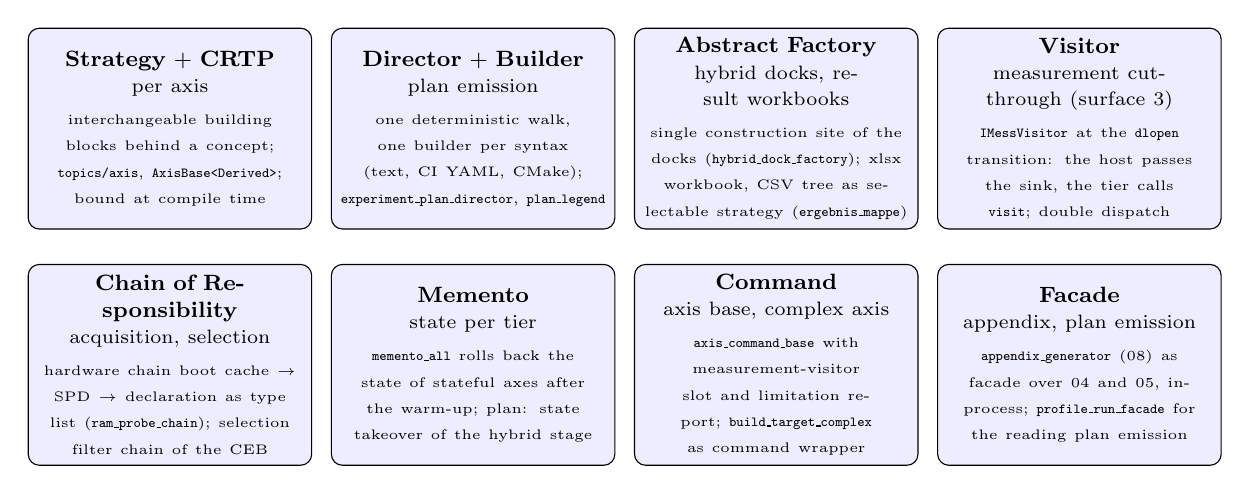
\begin{tikzpicture}[font=\footnotesize,
  mu/.style={draw,rounded corners,fill=blue!7,minimum width=3.6cm,minimum height=2.55cm,text width=3.4cm,align=center,inner sep=2pt}]
  \node[mu] (m1) at (0,0){\textbf{Strategy $+$ CRTP}\\{\scriptsize per axis}\\[2pt]{\tiny interchangeable building blocks behind a concept; \texttt{topics/axis}, \texttt{AxisBase<Derived>}; bound at compile time}};
  \node[mu] (m2) at (3.85,0){\textbf{Director $+$ Builder}\\{\scriptsize plan emission}\\[2pt]{\tiny one deterministic walk, one builder per syntax (text, CI YAML, CMake); \texttt{experiment\_plan\_director}, \texttt{plan\_legend}}};
  \node[mu] (m3) at (7.7,0){\textbf{Abstract Factory}\\{\scriptsize hybrid docks, result workbooks}\\[2pt]{\tiny single construction site of the docks (\texttt{hybrid\_dock\_factory}); xlsx workbook, CSV tree as selectable strategy (\texttt{ergebnis\_mappe})}};
  \node[mu] (m4) at (11.55,0){\textbf{Visitor}\\{\scriptsize measurement cut-through (surface 3)}\\[2pt]{\tiny \texttt{IMessVisitor} at the \texttt{dlopen} transition: the host passes the sink, the tier calls \texttt{visit}; double dispatch}};
  \node[mu] (m5) at (0,-3.0){\textbf{Chain of Responsibility}\\{\scriptsize acquisition, selection}\\[2pt]{\tiny hardware chain boot cache $\to$ SPD $\to$ declaration as type list (\texttt{ram\_probe\_chain}); selection filter chain of the CEB}};
  \node[mu] (m6) at (3.85,-3.0){\textbf{Memento}\\{\scriptsize state per tier}\\[2pt]{\tiny \texttt{memento\_all} rolls back the state of stateful axes after the warm-up; plan: state takeover of the hybrid stage}};
  \node[mu] (m7) at (7.7,-3.0){\textbf{Command}\\{\scriptsize axis base, complex axis}\\[2pt]{\tiny \texttt{axis\_command\_base} with measurement-visitor slot and limitation report; \texttt{build\_target\_complex} as command wrapper}};
  \node[mu] (m8) at (11.55,-3.0){\textbf{Facade}\\{\scriptsize appendix, plan emission}\\[2pt]{\tiny \texttt{appendix\_generator} (08) as facade over 04 and 05, in-process; \texttt{profile\_run\_facade} for the reading plan emission}};
\end{tikzpicture}
\caption[The register of design patterns]{The register of the design patterns of the apparatus (naming after Gamma et al.): per pattern
the role and the code location. All eight are executed at compile time --- binding via concepts, CRTP
and type lists instead of via virtual calls ---, because tier binaries may contain no runtime branching
between building blocks.}\label{fig:muster}
\end{figure}

The hybrid stage is the fourth carrier stage (Section~\ref{sec:heuristics-modes}); its code state lies
under \texttt{hybrid/} (Figure~\ref{fig:hybrid-dock}). Implemented are the dock contracts --- four
contract forms \texttt{standard}, \texttt{rollback}, \texttt{scan} and \texttt{resource\_control} as a
\texttt{constexpr} registry with sixteen status constants (\texttt{ok} and fifteen named rejection
reasons) ---, the minimal probe dock, the dock factory as the single construction site, the dock array
with \texttt{HybridDockVariant} (the one permitted variant site, Section~\ref{sec:axes-impl}) and the
runtime cap \texttt{max\_docks}, which rejects the $(N+1)$-th docking with \enquote{array full}, the
parser of the \texttt{<hybrid\_tier>} section (two-way switch \texttt{enabled}, exclusive per chain,
\texttt{max\_docks} mandatory with the stage switched on) and the binary proxy, which makes a hybrid
.so an ordinary tier binary to the outside: it satisfies \texttt{IAnatomyBase}, holds the dock array
and passes the drive through to the target that sits at a dock. Not implemented are the \texttt{.so}
export of the hybrid stage (it depends on an open layering requirement, because a hybrid \texttt{.so} would
have to link builder code), the eviction and the router (it needs actual measurement curves). Measured
against the file list that the \texttt{README} of the directory \texttt{hybrid/} envisages for the
dock, proxy and router layer, six of the nine files are implemented (dock contracts, probe dock, dock
factory, dock array, XML parser, binary proxy) and three are not (the tier module of the \texttt{.so}
export --- the two module sources under \texttt{tests/unit} demonstrate only the buildability of the
module ABI ---, the eviction and the router); besides these, the directory carries the four headers of
the classification layer (classification, concept gate, strategy per genus, synthesis matrix) and three
further headers for docking, the module ABI and the stamp chain, thirteen headers in total.
The Hybrid Module ABI v1 exports the same mandatory symbols as the plain tiers including family and
genus, and \texttt{comdare\_anatomy\_genus} reports the \emph{target} genus (what the module is for the
caller), never the reroute genus of the classification --- the same family-independent loader loads
the hybrid \texttt{.so} via the one loading route; the stamp chain of the hybrid stage and the hybrid positions
of the measurement-gate member (\texttt{hm}/\texttt{hmi}) carry its identity, and the genus build
admission carries six entries, the sixth for the reroute genus with the dock cap (default 32) as arity.
The hybrid live ranking is planned as the fourth evaluation component of the compare stage, and the
state reconciliation of the hybrid stage is planned via memento with two release artefacts, single and
hybrid, in the store (Section~\ref{sec:heuristics-modes}); implementation status: neither is
implemented, nor is the fix of the schema drift that the XSD does not carry the \texttt{<hybrid\_tier>}
section. The hybrid mode compiles only with the help of the CEB\@.
\begin{figure}[htbp]\centering
\begin{tikzpicture}[font=\footnotesize,>=Stealth,
  hb/.style={draw,rounded corners,fill=blue!7,text width=2.9cm,minimum height=1.0cm,align=center,inner sep=2pt,font=\scriptsize},
  dk/.style={draw,rounded corners,fill=orange!12,text width=1.95cm,minimum height=1.1cm,align=center,inner sep=2pt,font=\tiny},
  ex/.style={draw,rounded corners,fill=green!8,text width=2.6cm,minimum height=1.0cm,align=center,inner sep=2pt,font=\tiny}]
  \node[draw,rounded corners,dashed,minimum width=9.0cm,minimum height=5.4cm] (frame) at (0,-0.4){};
  \node[font=\bfseries\scriptsize,anchor=north west] at (-4.5,2.3){Hybrid \texttt{.so} (family HeuristikAdapter, reroute genus)};
  \node[hb] (proxy) at (-2.4,0.9){\texttt{HybridBinaryProxy}\\satisfies \texttt{IAnatomyBase}; passes the drive through to the target dock};
  \node[hb] (arr) at (2.3,0.9){\texttt{DockArray\{\allowbreak max\_docks\}}\\\texttt{HybridDockVariant}: the one permitted variant site};
  \draw[->,thick] (proxy)--(arr);
  \node[dk] (d1) at (-3.2,-1.4){Dock 1\\contract \texttt{standard}\\$\to$ target tier};
  \node[dk] (d2) at (-1.0,-1.4){Dock 2\\contract \texttt{rollback}\\$\to$ target tier};
  \node[dk] (d3) at (1.2,-1.4){Dock 3\\contract \texttt{scan}\\$\to$ target tier};
  \node[dk] (d4) at (3.4,-1.4){Dock $N$\\contract \texttt{resource\_\allowbreak control}\\$\to$ target tier};
  \draw[->] (arr)--(d1); \draw[->] (arr)--(d2); \draw[->] (arr)--(d3); \draw[->] (arr)--(d4);
  \node[font=\tiny,text=red!60!black] at (0.1,-2.55){docking $N+1$: status \texttt{array\_voll} (runtime cap \texttt{max\_docks})};
  \node[ex] (fac) at (-6.3,0.9){\texttt{HybridDockFactory}\\Abstract Factory: single construction site of the docks};
  \draw[->,dashed] (fac)--(proxy);
  \node[ex] (xml) at (-6.3,-1.4){\texttt{<hybrid\_tier enabled=true max\_docks=N>}\\parser: \texttt{enabled} exclusive per chain, \texttt{max\_docks} mandatory};
  \draw[->,dashed] (xml)--(d1);
  \node[ex] (sym) at (6.3,0.9){exports: seven mandatory symbols as for plain tiers; \texttt{genus()} reports the target genus (route C)};
  \draw[->,dashed] (frame.east)--(sym);
  \node[ex] (st) at (6.3,-1.4){stamp chain of the hybrid stage; measurement-gate fields \texttt{hm}/\texttt{hmi}; genus build admission: 6th entry};
\end{tikzpicture}
\caption[The hybrid stage in code]{The hybrid stage in code: the binary proxy makes the hybrid \texttt{.so} an ordinary tier binary to the
outside and holds the dock array with the runtime cap \texttt{max\_docks}; per dock one of four
contracts applies, the dock factory is the single construction site, the \texttt{<hybrid\_tier>}
section of the XML switches the stage and sets the cap. The exports are spelled identically to the
plain tiers, \texttt{genus()} reports the target genus. Not implemented: \texttt{.so} export,
eviction, router.}\label{fig:hybrid-dock}
\end{figure}

The store (Section~\ref{sec:lager}) has in code a compile-time-static key schema
(\texttt{bestand\_\allowbreak{}schluessel\_\allowbreak{}schema}) that declares the four stocks without
itself implementing store mechanics: stock~1, the binaries, is keyed via a key policy whose single
SHA-512 key is identical to the tier fingerprint, the cell bracketed beside it; stock~2, the measured
values, via the 128-hex fingerprint of the measured binary and the hardware identity of the measuring
machine, the cell bracketed beside it and never fused into the digest; stock~3, the synthesis batches,
and stock~4, the solutions, are declared as a work step of the full expansion of the store
(Table~\ref{tab:lager-schluessel}). Drift between schema and mechanics breaks when the mechanics are
built, not only in the store. The version lock (\texttt{axis\_version.lock}, format v3, 719 records of
three lines each) binds every source file of the axes --- the heuristics headers and the overlay cut
over which the overlay member of the tier fingerprint hashes --- to its content digest and its stamped
algorithm version: a deviation between lock and discovery is a failure, a downgrade of a
version-bearing header to digest-only is a failure without a write path, an upgrade is legitimate and
demands the deliberate regeneration of the lock; the CI gate \texttt{contract:axis-version-lock}
enforces this. From the schema follow the store properties of the concept: the measurement is always
switched on, in the store only what is missing there is re-measured; a version change of an axis
changes stamp and fingerprint and rebuilds the affected store stack; and because the hardware identity
stands in the measured-value key, every machine type has its own stock of measured values.
Implementation status: schema, lock and the stocks~1 and~2 are implemented; the full expansion ---
planner leaf function, CEB full placement, hybrid storage, commit skip, rebuild flag, XML target choice
--- and the binaries with and without measurement sensors together with curve files as store entries
are planned but not implemented.
\begin{table}[htbp]\centering\footnotesize
\begin{tabular}{@{}lp{6.2cm}p{3.0cm}p{2.6cm}@{}}
\toprule
Stock & Key components & Source in code & Implementation status \\
\midrule
1 binaries & the one SHA-512 key ($=$ tier fingerprint); cell bracket beside it & key policy of the stock log & implemented \\
2 measured values & 128-hex fingerprint of the measured binary; hardware identity of the measuring machine; cell bracketed beside it, never fused & measured-value key source of the stock log & implemented \\
3 synthesis batches & machine; full stamp; reference to measurement level and channel & schema declared & not implemented (full expansion) \\
4 solutions & canonicalized hash of the user XML\@; machine; references to the participating stocks & schema declared & not implemented (full expansion) \\
\bottomrule
\end{tabular}
\caption{The four store stocks and their key components according to the compile-time-static key
schema; the version lock binds the axis sources to digest and stamped
version.}\label{tab:lager-schluessel}
\end{table}

With this, the apparatus is fully described --- from the four repositories through the probe, the
eighteen organ axes and the carrier-stage chain to the chain from plan to tier binary, its contract
surfaces, the layer-wise quality assurance, the realm roots in code, the pattern register, the hybrid
stage and the store. Chapter~\ref{ch:eval} lays out the methodology by which this apparatus is
assessed.
